%%% DOWNLOADED, EDITED AND COMPILED ON COMPUTER
%\documentclass[jou,11pt]{apa7}
\documentclass{foushee-adapted-preprint}
\usepackage{lipsum}
\usepackage[american]{babel}
\usepackage{csquotes}
\usepackage[colorinlistoftodos]{todonotes}
\usepackage{paralist}
\usepackage{booktabs}
\usepackage{setspace}
%\usepackage{longtable}
\usepackage{microtype}
\usepackage{multirow}
\usepackage{adjustbox}
\usepackage{array}
\usepackage{xcolor,colortbl}
\usepackage{threeparttable}
\usepackage{rotating}
\usepackage{caption}
\leadauthor{Foushee} 
\definecolor{lightgreen}{rgb}{0.698, 0.8745, 0.5412}
\definecolor{lightergreen}{cmyk}{.20, 0, .38, 0} %0.13
\usepackage{hyperref} 
\hypersetup{colorlinks=true,
    urlcolor=livingcoral,
    anchorcolor=livingcoral,
    citecolor=livingcoral,
    filecolor=livingcoral} 
\addbibresource{bibliography.bib}
%0.9\baselineskip
\setlength{\parskip}{0.5\baselineskip}
\usepackage{titlesec}
\newcommand{\fulllanguagestab}{S1}

\newcommand{\geomeanstab}{S2}
\newcommand{\religionmeanstab}{S3}
\newcommand{\wealthmeanstab}{S4}
\newcommand{\faceaudiomeanstab}{S5}
\newcommand{\facelabelmeanstab}{S6}
\newcommand{\learningmeanstab}{S7}


\newcommand{\geomodeltab}{S8}
\newcommand{\religionmodeltab}{S9}
\newcommand{\religionchirelmodeltab}{S10}
\newcommand{\faceaudiomodeltab}{S11}
\newcommand{\facelabelmodeltab}{S12}

\newcommand{\facemodalitytab}{S13}
\newcommand{\faceenglishmodalitytab}{S14}

\newcommand{\wealthmodeltab}{S15}
\newcommand{\learningmodeltabs}{S16--S20}

\newcommand{\geofamtab}{S21}
\newcommand{\relfamtab}{S22}
\newcommand{\faceaudiofamtab}{S23}
\newcommand{\facelabelfamtab}{S24}
%\newcommand{\wealthfamtab}{S25}
%\newcommand{\learningfamtab}{S21}

\newcommand{\geogendertab}{S25}
\newcommand{\relgendertab}{S26}
\newcommand{\wealthgendertab}{S27}
\newcommand{\faceaudiogendertab}{S28}
\newcommand{\facelabelgendertab}{S29}
%\newcommand{\wealthfamtab}{S25}

%FIGURES
\newcommand{\nonengbarplot}{S1}
\newcommand{\engbarplot}{S2}

\begin{document}
\title{Sociolinguistic development in a diverse, multilinguistic environment: Evidence from multilingual children in Gujarat, India}
\shorttitle{{Socio-Multilinguistic Development}}

\author[1,2, \Letter]{Ruthe Foushee}
\author[2]{Sophie Regan}
\author[2]{Roya Baharloo}
\author[2]{Mahesh Srinivasan}

\affil[1]{Department of Psychology, New School for Social Research, 80 $5^{\textnormal{th}}$ Avenue, New York, NY 10011}
\affil[2]{Department of Psychology, University of California, Berkeley, 2121 Berkeley Way West, Berkeley, CA 95720}
\maketitle
%\addbibresource{bibliography.bib}
%0.9\baselineskip
\begin{abstract}
\noindent
In today's pluralistic societies, children regularly acquire multiple languages and are exposed to an even larger set of languages spoken by others in their environment. Yet despite the prevalence of multilingualism globally, most research on sociolinguistic development has focused on monolingual children in environments with relatively little linguistic diversity, and as such has left questions of what children take different languages to socially signify largely unaddressed. The present study aimed to fill this gap by tracing the development of social inferences about different languages among 129 multilingual 7- to 13-year-olds in Gujarat, India. Contrary to the prediction that children in multilingual contexts should be unlikely to make stereotyping inferences about a person speaking a language (e.g., because they might expect the person to know additional languages), children in our sample selectively linked the different languages and language varieties that we probed (Gujarati, Marathi, Hindi, Urdu, Tamil, American English, Indian English, and Mandarin Chinese) with different social dimensions---including facial appearance, geographic origin, religion, and wealth. Children's responses generally reflected associations grounded in real-world regularities, but also reflected some associations that do not have a real-world basis (e.g., judging that Indian English speakers tend to be white, Christian, and originate from outside of India). %These associations became more reliable with age, and o
Older children were also more likely to predict different languages to be differentially learnable by individuals of specific ethnicities, exhibiting a kind of essentialist belief. We discuss our findings in light of the sociolinguistic study of \textit{personae}.
\end{abstract}
\begin{corrauthor}
ruthe\at newschool.edu
\end{corrauthor}
\begin{keywords}
\noindent
\textit{multilingualism} | \textit{sociolinguistic development} | \textit{linguistic essentialism} | \textit{linguistic diversity} | \textit{dialect perception} | \textit{language attitudes} | \textit{personae}
%\textit{dialectal diversity} | \textit{social categorization} | \textit{personae}
\end{keywords}
\vspace{-5pt}
\begin{pubcitation}
Foushee, R., Regan, S., Baharloo, R., \& Srinivasan, M. (\textit{in press}). Sociolinguistic development in a diverse, multilinguistic environment: Evidence from multilingual children in Gujarat, India. Multilingualism [Special issue]. \textit{Cognitive Development}.
\end{pubcitation}
\maketitle
\vspace{5pt}
%\section*{Introduction}
%\authornote{
%{\vspace{-10pt}  }\\
%    \addORCIDlink{Ruthe Foushee}{0000-0002-8361-1725}\\
%   \addORCIDlink{Sophie Regan}{0009-0006-3061-9906}\\
%   \addORCIDlink{Roya Baharloo}{0000-0003-3062-6891}\\
%   \addORCIDlink{Mahesh Srinivasan}{0000-0003-0350-2703}\\
%   Correspondence concerning this article should be addressed to Ruthe Foushee (ruthe@newschool.edu).}
%\section{Introduction}
\lettrine{I}n today's increasingly pluralistic societies, children regularly acquire multiple languages and are routinely exposed to an even larger set of languages spoken by others in their community \parencite{lin2020research, grosjean2010bilingual}. 
For example, children in Gujarat, India---the site of the present study---often acquire or have significant exposure to the local regional language (e.g., Gujarati), official languages of the government and schools (e.g., Hindi and Indian English), languages spoken by family members who may have originated from other regions in India (e.g., Marathi, Punjabi, Tamil), and languages spoken by religious sub-communities (e.g., Urdu), among others. Given the widespread presence of linguistic diversity in children's environments, it is important to understand how children make sense of such variation: What kinds of social inferences do children make about individuals on the basis of the language(s) they speak, and how might this change over development? %as they grow older

Despite the prevalence of multilingualism globally, most research on sociolinguistic development has focused on monolingual children in environments with relatively little linguistic diversity (e.g., \cite{moon1993two, kinzler2007native, shutts2009social, buttelmann2013selective, weatherhead2019preschoolers}). What children take different languages within the same environment to socially signify has largely been left unaddressed. The present study begins to fill this gap by tracing the development of beliefs and social inferences about language---including essentialist beliefs about language-learning, and inferences about speakers of different languages' facial appearance, geographic origin, wealth, and religion---among 7- to 13-year-old multilingual children in Gujarat, India.

\subsection*{Prior Work in Sociolinguistic Development}
Prior work conducted in Western contexts suggests that from infancy children use language as a marker of social group, expecting individuals who speak a common language to affiliate with one another and share preferences \parencite{liberman2017preverbal,liberman2016early}. Language also appears to be a key dimension along which infants and preschoolers draw ingroup/outgroup boundaries, as they prefer to look at \parencite{kinzler2007native}, imitate \parencite{buttelmann2013selective}, and accept toys or food from speakers of their own language and accent, compared to speakers of different languages or varieties \parencite{kinzler2007native,shutts2009social}. Reflecting the strength of their beliefs about the connection between language and social identity, U.S. English-speaking preschoolers also appear to essentialize language---viewing it as something that is stable and biologically inherited (e.g., expecting a child adopted at birth to speak the language of their birth parents rather than of their adopted parents; \cite{hirschfeld1997young}; see also \cite{kinzler2012children}).  

Perhaps because the majority of prior work has been conducted in contexts among monolingual children with little linguistic diversity, when prior studies have explored the inferences that children make about speakers of different languages, they have typically contrasted speakers of a familiar language with speakers of a single, unfamiliar language (e.g., \cite{liberman2017preverbal, hirschfeld1997young, kinzler2012children, kinzler2007native, moon1993two, wagner2014children}), or have instead focused on speakers of different varieties of the same language (e.g., \cite{weatherhead2019preschoolers, mccullough2019regional, kinzler2013northern}). 
For example, Hirschfeld and Gelman (\citeyear{hirschfeld1997young}) found that U.S. preschoolers assumed that individuals who spoke a different language from English would be more likely to be  of a minority race, wear different clothes, and live in different-looking dwellings. In support of the idea that children gradually develop more selective sociolinguistic inferences---i.e., beyond simply assuming that speakers of a different language will be different from them---older U.S. children make more specific inferences about a speaker's geographic origin and personality on the basis of their dialect or accent \parencite{mccullough2019regional,kinzler2013northern}.

\subsection*{Sociolinguistic Development in a Multilinguistic Environment}
Taken together, this prior work on sociolinguistic development---conducted largely with Western, monolingual samples---has suggested that children can make a limited number of social inferences from a small number of linguistic distinctions (e.g., judging speakers with Southern English accents as ``nice'' and speakers with Northern accents as ``smart;'' \cite{kinzler2013northern}). 
But how might multilingualism, and the presence of high levels of diversity in terms of both named languages and language dialects, within children's linguistic environments, shape their social associations involving language? %(and potentially complicate or refine) 
Given the lack of prior work on this topic, our approach was exploratory, and considered the following alternative hypotheses: on the one hand, one might expect multilingual children in contexts with high linguistic diversity 
\begin{inparaenum}[(1)]
    \item to be less likely to essentialize language (i.e., as they will have had more first-hand experience observing that languages are learned) and
    \item to make fewer stereotyping assumptions about a person based on the language they are speaking (i.e., as children in these contexts are likely to understand that a person can know multiple languages, beyond the one they are currently using).
\end{inparaenum} 
Indeed, consistent with this prediction of reduced essentialism, one prior study found that while monolingual and simultaneous bilingual children expected a baby to speak their biological parents' language, sequential bilinguals (who learned a second language after age three) were less likely to endorse this essentialist belief (\cite{byers2015bilingualism}; see also \cite{dautel2018once}).

On the other hand, it is also possible that even within a multilingual environment, children may leverage the social cues that language can provide, relying on language as a simple heuristic to make sense of a complex social landscape. From this perspective, one might expect multilingual children in contexts of high linguistic diversity to develop selective and nuanced associations with the many different languages they encounter, across a variety of dimensions (e.g., making language-based inferences about physical appearance, geographic origin, social class, personality, and more), going beyond the smaller set of inferences documented in less multilingual contexts. 
Indeed, consistent with this account, one study found that South Indian 5- to 10-year-old Tamil-speaking children who had some exposure to Hindi and English reliably judged Tamil speakers to be ``most Indian,'' ``most kind,'' and ``most intelligent,'' relative to speakers of Hindi, British English, and Indian English \parencite{santhanagopalan2021nationality}. %Although these results could be explained by a simple familiarity bias (leading to more positive impressions of speakers of the local language, Tamil), children did not judge Tamil speakers to be the ``best leaders'', perhaps reflecting their sensitivity to the relative status and power of the Tamil community within India and the world. 

The present study builds on this prior work to assess the range of sociolinguistic associations that multilingual children in multilingual environments may develop. 
We were especially interested in extending beyond language attitudes and general evaluative judgments of speakers (e.g., of their warmth and competence) toward assessing children's context-specific associations with different languages. 
Having a positive view of Tamil speakers, for example, might predict that one would regard them as ``kind'' and ``intelligent'' \parencite{santhanagopalan2021nationality}, without generating any clear prediction about such speakers' geographic origin, religion, appearance, or wealth. %where they come from, their religion,  geographic origin, religion, facial appearance, or wealth of such speakers. 
The present study was interested specifically in children's tendency to make the latter kind of substantive inferences, as well as the mechanisms that may give rise to these inferences over development.

\subsection*{The Present Study and Context}
We explored the development of sociolinguistic associations and essentialist beliefs about language among 129 multilingual children and adolescents (mean age = 11 years, SD = 1.6) from a diverse, multilingual context within the city of Vadodara, in Gujarat Province, India. 
Our participants attended an English-medium school and reported using an average of 3.8 languages (see \textit{Participants}). 
Children in Gujarat acquire, use, and hear diverse languages across multiple distinct contexts, each potentially offering insights into a speaker's heritage, experience, and affiliations. 
India has many regional languages, which may be spoken in the home and can indicate an individual's (family's) region of origin. 
%As the regional language of Gujarat, 
For example, Gujarati is described as the ``mother tongue'' of about 86\% of Gujarat's population \parencite{india2011census}. 
Marathi, the regional language of the neighboring state of Maharashtra, is less ubiquitous, but often spoken in the homes of Gujarat residents originally from Maharashtra---indeed, Gujarat has the third-largest population of Marathi-speakers outside of the state. 
While Hindi is identified as the ``mother tongue'' of only 7\% of Gujarat's population, it is commonly used in public spaces because it is one of the government's official languages (and one of the languages formally taught in schools). 
Urdu, which differs little from Hindi phonetically, is listed as a native language by just 1\% of individuals in Gujarat. While both Urdu and Hindi are considered standard registers of a common language, Hindustani, they use different scripts and vocabulary, and Urdu is strongly associated with Muslims across India.  
Finally, while English is listed as a native language by only 0.007\% of Gujarat's population, its prominence in government, academic institutions, and media---including as the medium of instruction at the school that our participants attended---ensures that Gujarati children have experience English as well. 
%Finally, about 1\% of individuals in Gujarat list Urdu as their native language. 
%Urdu is strongly associated with Muslims across India.  
%which most often included Gujarati (the local regional language), Hindi (the language of the government and lingua franca in North India), and Indian English (the language of instruction at their school), in addition to family heritage languages (e.g., Marathi, Punjabi, Urdu, Tamil). 

Here, we presented participants with questions regarding eight languages or dialects that crossed regional, political, ethnic, and religious boundaries. 
To avoid forcing stereotyping, participants could always `opt out' of answering a question or could select more than one response to a question. Together, our measures 
\begin{inparaenum}[(1)]
    \item assessed whether children---when presented with unlabeled audio clips (e.g., a clip in Hindi that we did not label as ``Hindi'')---associated speakers of each language or variety with a particular geographic region of origin, religion, level of wealth, and an ethnically- or religiously-stereotypical facial appearance, and
    \item probed whether children essentialized language in predicting that individuals of different ethnic or religious identities would vary in their ability to learn a particular language.
\end{inparaenum} 
Lastly, we measured children's recognition of each language by asking them to produce the name of each language after listening to a representative audio clip. %its corresponding audio clip.

As a first step toward assessing the mechanisms through which children develop associations with different languages, we asked participants to guess the facial appearance of speakers in two ways: when hearing unlabeled audio samples of the language (as noted above), and, in a later block, when using the language name (e.g., ``Who speaks \textit{Tamil}?''). 
We reasoned that, while responses to unlabeled audio clips alone could reflect children's ``bottom-up'' environmental experience (e.g., hearing Tamil in their environments and associating it with individuals of a particular appearance), queries involving language names would additionally allow children to leverage ``top-down'' conceptual knowledge acquired via cultural transmission (e.g., stereotypes about ``Tamil'' speakers communicated by parents), that they may not be able to access from the unlabeled audio clips alone (e.g., if they did not recognize the audio clip as containing ``Tamil'').

\section{Method}
\subsection{Participants}
Participants were 129 students at an English-medium school in Vadodara, Gujarat, India (65 female, 64 male, 65 Hindu, 58 Muslim, 7.7--13 years of age, $M_{age}=11$, $SD_{age}=1.6$). 
We tested children across three grades: 3$^{\textnormal{rd}}$ ($n=27$, 13 female, 14 male, 10 Hindu, 16 Muslim; 7.7--9 years, $M_{age}=8.22$, $SD_{age}=0.31$), 5$^{\textnormal{th}}$ ($n=55$, 29 female, 26 male, 30 Hindu, 22 Muslim; 9.70--11 years, $M_{age}=10.30$, $SD_{age}=0.47$), and 7$^{\textnormal{th}}$ ($n=48$, 23 female, 24 male, 24 Hindu, 20 Muslim; 12--13 years, $M_{age}=12.4$, $SD_{age}=0.49$). 
To probe productive and receptive multilingualism in this sample, children were asked a number of questions that encouraged them to list languages that they had experience with, including
\begin{inparaenum}[(1)]
    \item their ``mother tongue,''
    \item the languages they speak,
    \item the languages they understand,
    \item the languages they use at home, and
    \item the languages they use with their friends
\end{inparaenum} (see Table~\fulllanguagestab\ for tabulated response data). %for full response data, see \textit{Supplementary Online Materials}). 
In response to all of these questions combined, children listed an average of 3.8 languages (\textit{range}=1--8, \textit{Med}=4), with a total of 9 unique languages identified as their ``mother tongue,'' 11 unique languages that they reported speaking or using at home, 16 unique languages they reported as understanding, and 6 unique languages used with friends (see Table~\ref{tab:child-langs}).%The set of languages included Hindi ($n=122$), Gujarati ($n=117$), English ($n=106$), Marathi ($n=59$), Urdu ($n=23$), Punjabi ($n=11$), Sindhi ($n=5$), and Tamil ($n=4$).
\footnote{A shortcoming of this approach to measuring multilingual experience is that it relies on self-reporting by young children. For example, the number of children who reported experience using English was 106 (meaning that 23 of the total 129 participants did not list English), even though all participants had experience with English (being students at an English-medium school). 
We suspect that participants who did not list English likely did not do so because the survey was being conducted in English and so they may have taken it as unnecessary to list English.} 

% latex table generated in R 4.3.2 by xtable 1.8-4 package
% Mon Jun  3 00:53:35 2024
\begin{table}[t]
\caption{Languages Reported as Spoken or Understood by \textgreater1 Child}\label{tab:child-langs}
\centering
\begin{threeparttable}
\begin{tabular}{p{3cm}c}
\toprule
%\multirow[b]{2}{*}{\textbf{Language}} & \multirow[c]{2}{1.5cm}{\centering\bfseries\textit{n} children} \\ 
%&\\
\textbf{Language} & \bfseries\textit{n} children\\
\midrule
\rowcolor{lightergreen}Hindi & 122 \\ 
\rowcolor{lightergreen}Gujarati & 117 \\ 
\rowcolor{lightergreen}English & 106 \\ 
\rowcolor{lightergreen}Marathi &  59 \\ 
\rowcolor{lightergreen}Urdu &  23 \\ 
Punjabi &  11 \\ 
Sindhi &   5 \\ 
\rowcolor{lightergreen}Tamil &   4 \\ 
Bengali &   3 \\ 
%Arabic &   2 \\ 
%Marwari &   2 \\ 
%Rajasthani &   2 \\ 
%Sanskrit &   2 \\ 
\bottomrule
%\multicolumn{2}{l}{\textit{Note.} %The following languages were listed by two children: Arabic, Marwari, Rajasthani, Sanskrit}
\end{tabular}

\begin{tablenotes}[normal, flushleft]
\small
\vspace{5pt}
     % \item An additional 4 languages were listed by 2 children: Arabic, Marwari, Rajasthani, Sanskrit
      %\item \textit{Listed by 2 children}: Arabic, Marwari, Rajasthani, Sanskrit\\%(\textit{n}=2)\\%; Bihari, French, Kathiyawadi, Malyam, Memon, Polish, Telgu (\textit{n}=1).
      \item \textit{Notes.} {Highlighted rows indicate languages included in the study.}\\ 
      \textit{Additional languages listed by 2 children}: Arabic, Marwari, Rajasthani, Sanskrit\\
    \end{tablenotes}
  \end{threeparttable}
\end{table}
%Bihari, French, Kathiyawadi, Malyam, Memon, Polish, Telgu

The study was conducted in January 2019 by an English-speaking researcher from the U.S. (RF) and two English-speaking researchers from Gujarat who also spoke both Gujarati and Hindi, along with either Marathi or Urdu. 
All participants were tested by the same set of researchers. 
Students took part in the study in groups of 4--12, depending on their age: 7$^{\textnormal{th}}$-graders participated in groups of 8$-$12, while 3$^{\textnormal{rd}}$$-$5$^{\textnormal{th}}$--graders participated in groups of 4$-$8. Researchers read aloud and explained each survey question, one-by-one, to the group of children, waiting for all children to individually indicate their response on paper before moving on to the next question. 
Questions were presented in English but multilingual researchers provided clarification in other languages if needed.
%As all students in each testing group received survey questions in the same order, we sought to ensure that each testing group was composed of roughly even numbers of girls and boys, and Hindus and Muslims (estimated by local research assistants based on the child's name for recruitment purposes, but provided by the child directly during the study session). 
All stimuli can be found at the online repository for this study: \url{https://osf.io/xa6h3/?view_only=45b0f9d03e664ce18cdfedf5c2b2aa2f}. 

\begin{figure*}
    \centering
    \includegraphics[width=\linewidth]{figures/2024-IndiaSocioling-Final.pdf}
    \caption{\textit{Study Method.} 
    Children's associations, beliefs, and identification of the languages we tested were probed via four blocks of questions, the first three of which (\textit{Speaker Associations}, \textit{Stereotypical Speaker Selection}, and \textit{Linguistic Essentialism}) were counterbalanced across children.
    While children saw (and heard) both male and female speakers, only the female face array is shown here (face selections were coded as: \textsc{Muslim}, \textsc{Hindu}, \textsc{Dravidian}, \textsc{Asian}, \textsc{White}, and \textsc{No opinion}).  %of questions eliciting categorical, ordinal, and open-ended responses.
    }
    \label{fig:method}
\end{figure*}
\subsection{Stimuli}
We tested children's recognition of and associations with eight languages or varieties representing multiple language families and crossing regional, political, ethnic, and religious boundaries: Gujarati, Hindi, Urdu, Marathi, Tamil, Indian English, U.S. English (`Mainstream' American English), and Mandarin. 
We will henceforth refer to these as ``languages.'' 
When languages were queried by name, rather than presented in an unlabeled audio clip, the number of languages reduced to seven, as Indian and U.S. English were both referred to as ``English.'' 
The other languages were referred to as ``Gujarati,'' ``Hindi,'' ``Urdu,'' ``Marathi,'' ``Tamil,'' and ``Chinese.'' 

\subsubsection{Auditory Stimuli.}
We recorded audio clips from a male and female speaker of each of the eight languages (16 clips total). 
Speakers produced a sentence from their language or variety with the meaning ``They will read the book soon.'' 
This sentence was selected because it is short and highlights phonological and lexical distinctions across the languages, including distinctions between highly similar languages like Hindi and Urdu. 

\subsubsection{Visual Stimuli.}
Visual stimuli included arrays of five faces, intended to stereotypically represent five ethnic and religious identities: North Indian Hindu, Muslim, South Indian (Dravidian) Hindu, white, and East Asian. 
Where possible, faces were taken from an online set of `averaged' faces by nationality (composite images aligning many faces from each country to obtain an average face; \url{faceresearch.org}), and were otherwise found via internet image search, in consultation with research assistants. 
There were two arrays of faces---one depicting only men, the other depicting only women. Each array consisted of the following types: 
\begin{inparaenum}[(1)]
    \item \textsc{Hindu}: an averaged `Indian' woman wearing a bindhi or an averaged `Indian' man,
    \item \textsc{Muslim}: a woman with her head covered or a man wearing a topi cap and keffiyeh,
    \item \textsc{Dravidian}: a South Indian woman wearing a bindhi or a South Indian man,
    \item \textsc{White}: a white woman with light brown hair or an averaged `white American' man, and
    \item \textsc{Asian}:  an averaged `Chinese' woman or an averaged `Chinese' man. 
\end{inparaenum}
To avoid forcing children to make stereotyping selections, children could always select more than one face or a final option: \textsc{No Opinion} (see Figure~\ref{fig:method}).

\subsection{Procedure}
The study consisted of four blocks (Figure~\ref{fig:method}). 
The first three blocks---\textit{Speaker Associations}, \textit{Stereotypical Speaker Selection}, and \textit{Linguistic Essentialism}---were counterbalanced across participants, while the \textit{Language Identification} block always came last. 
Children were probed about speaker associations and stereotypical speaker selections using two audio clips for each language---one by a male speaker and one by a female speaker.
They likewise made stereotypical speaker selections for each language using two face arrays---one female and one male. 
The order in which the genders of speakers was presented was counterbalanced, such that half of children responded first about the female speakers in every relevant block, and the other half responded first about the male speakers. 
%When children were asked to make stereotypical speaker selections using language labels (e.g., ``who speaks \textit{English}?''), they answered for all languages using one face array---e.g., the female face array---then for the other face array---e.g.,   two face arrays for each language---one male and one female---and the order was also counterbalanced. 

\subsubsection{Speaker Associations.}
Children heard unlabeled audio samples of each of the eight languages in a female and male voice (16 trials total). 
For each clip, children judged the speaker's geographic origin, religion, and wealth. 
\textit{Geographic origin} was judged by selecting from among four options in response to the prompt ``This speaker is from\ldots'': 
\begin{inparaenum}[(a)]
    \item Gujarat (Same place as me),
    \item Another part of India (A different city),
    \item Outside India (Foreign), or
    \item No opinion. 
\end{inparaenum}
\textit{Religion} was judged by selecting from among six options with the prompt ``This speaker's religion is\ldots'': 
\begin{inparaenum}[(a)]
    \item Hindu,
    \item Muslim,
    \item Jain,
    \item Buddhist,
    \item Christian, or
    \item No opinion. 
\end{inparaenum}
\textit{Wealth} was judged by selecting from among four options with the prompt ``This speaker has\ldots'': 
\begin{inparaenum}[(a)]
    \item Less money than the people in my city,
    \item As much money as the people in my city,
    \item More money than the people in my city, or 
    \item No opinion. 
\end{inparaenum}

\subsubsection{Stereotypical Speaker Selection.}
In the \textsc{Audio} block---which always came first---children heard a clip of each language and were asked who ``could be speaking'' from an array of five stereotypical faces (always matched to the apparent gender of the speaker in the audio clip). 
There were 16 trials (8 female voice/face trials, 8 male voice/face trials). 
In the \textsc{Language Name} block, children instead selected possible speakers when asked about each language by \textit{name}: e.g., ``Who speaks \textit{Hindi}?'' (14 trials total: 7 for the female face array, 7 for the male). 
Children were told that they could choose more than one face or select ``No opinion.'' 

\subsubsection{Linguistic Essentialism.} 
In the \textit{Linguistic Essentialism} block, children responded to a combination of Likert-scale, rating, and open-ended questions probing their intuitions about the learnability of languages by members of different ethnic, religious, and regional groups. 
We focus our analysis on a subset of these questions, where children were presented with the face arrays (half of children saw the female face array, and half saw the male face array), and asked to imagine that the people shown in the pictures were all the same age and had all lived on the same street for their entire lives. 
Then, they were asked to judge how well each person would ``come to learn'' each language if they had never heard or spoken it before but went to study it now (e.g., ``How well will which each of these women come to speak \textit{Hindi}? Remember, they do not speak it now.''). 
Participants selected from among four options for each face:
\begin{inparaenum}[(a)]
    \item {Not at all (0\%)},
    \item {Medium (50\%)},
    \item {Very well (100\%)}, or 
    \item {No opinion}. 
\end{inparaenum}
Our approach here was similar to that of Sun and colleagues (\citeyear{sun2023essentialist}), who adapted the classic linguistic essentialism task of Hirschfeld and Gelman (\citeyear{hirschfeld1997young}) by presenting adult participants with a scenario in which a baby was adopted from a Korean monolingual family into an %American 
English-only environment. Instead of asking whether the baby would grow up speaking Korean, as Hirschfeld and Gelman had asked preschoolers---and which older participants may immediately reject if they understand that some exposure to a language is required to learn it---Sun and colleagues (\citeyear{sun2023essentialist}) asked whether, when the baby in this scenario went to high school, they would be better at learning Korean than other students who did not have Korean ancestry. 
Our approach was thus similar to Sun and colleagues (\citeyear{sun2023essentialist}) in probing whether participants believed that individuals would vary in their ability to learn a new language, but it differed in that we only presented participants with information about the appearance of the individuals in question %, and thus about their likely ethnic identity 
(as opposed to telling participants about the language background of those individuals' birth parents).% and presenting a switched-at-birth scenario).
\footnote{A drawback of our approach is that ``essentialist'' responding in our task requires the participant to draw on an association between the appearance of the individual, their likely ethnicity, and the language associated with that ethnicity (e.g., to recognize that East Asian people often speak Mandarin). 
However, this indirect approach arguably also confers a benefit in that participants are not given any explicit information intimating that the individuals in question might have an advantage at learning that language (because we do not explicitly tell participants anything about the language spoken by the learners' ancestors).}  

\subsubsection{Language Identification.}
In the final block, children were asked to write the name of each language after listening to it a final time (half heard only the female audio clips, and half heard the male clips). Responses were coded as `0' (incorrect), or `1' (correct), ignoring spelling errors.
%The study ended with basic questions regarding children's own linguistic identities. %(see \textit{Supplementary Online Materials}).

\subsection{Analysis}
All analyses were conducted in R \parencite{R}. 
We report results from two classes of analyses. 
First, for questions eliciting an ordinal response (as in the case of speaker-wealth associations or predicted learning), we constructed mixed effects ordinal regression models using the \texttt{ordinal} library in R \parencite{R, ordinalR}.\footnote{Model syntax for wealth associations: \texttt{clmm(wealth\_rating $\sim$ 0 + language + child\_age + (1|child), link="logit")}; for learning predictions: \texttt{clmm(learning\_rating $\sim$ 0 + speaker\_face + child\_age + speaker\_face:child\_age + (1|child), link="logit")}}
Second, for questions eliciting categorical responses from a closed set of (unordered) response options (i.e., for questions about speakers' geographic origin, religion, and stereotypical appearance), we use mixed effects multinomial models (fit using the \texttt{mclogit} library; \cite{mclogit}), to predict the odds of selecting each meaningful and mutually exclusive response option (that is, excluding selections of multiple response options or of ``No opinion''), relative to a reference response (designated as the option selected by the greatest overall number of children for that response set). Each model included language, child age (in years, mean-centered), and their interaction where it improved model fit, along with random intercepts for each child.\footnote{Model syntax: \texttt{mblogit(response $\sim$ 0 + language + child\_age + language:child\_age, random=$\sim$1|child)}} % and each of the other response options (e.g., what factors predict indicating that a speaker is ``from another place in India'' as opposed to ``from Gujarat''---the reference level---or ``from outside of India'' as opposed to ``from Gujarat''). 
 
%We constructed two additional models for each 
For questions that asked children to select among the stereotypical speaker faces, we constructed two additional models to evaluate the effect of language presentation modality (audio vs. name). 
Because there were two language varieties presented auditorily (Indian English and U.S. English) corresponding to a single language name (``English''), we analyzed the non-English and English data separately. 
The first model predicted children's face selection from child age and the interaction of language (excluding English) and modality.\footnote{\texttt{mblogit(face $\sim$ 0 + child\_age + language + modality + language:modality, random=$\sim$1|child)}}  
The second model---restricted to the English data---predicted children's face selection given their age and a three-level factor combining language and modality (\textit{Indian English Audio} vs. \textit{U.S. English Audio} vs. \textit{English Name}).\footnote{\texttt{mblogit(face $\sim$ 0 + child\_age + english\_trial\_type, random=$\sim$1|child)}} 
%\footnote{Because ``English'' correspon we had two levels of the audio data for English [Indian English, American English] but only one level of the language name data [``English''], we dropped these data from this model, and conducted a separate model for these data).  %their interaction, and child religion as model predictors. 

For all multinomial models, we also conducted an additional analysis assessing the effects of participants' language \textit{familiarity} in predicting their responses. 
Language familiarity was operationalized via a composite variable capturing whether participants reported productive or receptive knowledge of a language, or could identify it by name in the \textit{Language Identification} block at the end of the study.  %\footnote{Because there was little to no variance in children's familiarity with Gujarati, Hindi, and Indian English, according to this composite measure, these data were dropped from this analysis.} 
The results of these analyses appear in full in the Supplement (Tables \geofamtab, \relfamtab, \faceaudiofamtab, and \facelabelfamtab). 

 

 %Finally, for questions eliciting a correct/incorrect response (i.e., language identification), we constructed mixed effects logit models using the R lme4 library \parencite{R, barr2013random}, and 
Our exposition relies on odds ratios, or \textit{ORs}, and 95\% bootstrapped confidence intervals (\textit{95\% CI}s), to selectively report the insights gained from our models (odds ratios whose confidence intervals do not include 1 are considered reliable), along with select descriptive details illustrating trends in children's response patterns. 
We use likelihood ratio tests comparing nested models with and without a given predictor using the \textttt{anova} command in R \parencite{R} to assess the significance of model terms. 
Full regression tables for all models are available in the Supplement, along with tables reporting additional analyses assessing the effects of speaker gender 
%The Supplement also includes regression tables from additional analyses assessing the effects of participants'  (i.e., a composite variable accounting for whether participants reported productive or receptive knowledge of a language, or could identify it by name in the Language Identification block at the end of the study), and stimuli gender 
(i.e., whether participants were responding to male or female voices, and whether they were selecting among male vs. female face arrays) on participants' responses (Tables~\geogendertab--\facelabelgendertab).

Deidentified data can be found at the online repository for this study (\url{https://osf.io/xa6h3/?view_only=45b0f9d03e664ce18cdfedf5c2b2aa2f}), and code for all analyses can be found at an be found at \url{https://github.com/foushee/india-socioling}.

\section{Results}
\subsection{Speaker Associations}
\subsubsection{Geographic Origin: This speaker is from\ldots} 
No child selected multiple geographic origins for the speaker of an audio clip. Twenty-seven children selected ``No opinion'' on at least one trial (39 total, including 9 in response to Mandarin, and 8 in response to Tamil). 
For all languages but Marathi, the response given by the majority of children in 3$^{\textnormal{rd}}$ grade was the same response given by the majority of children in 7$^{\textnormal{th}}$ grade, suggesting that children at the beginning of our age range have picked up on regularities between the language a person speaks and where they are from.\footnote{For Marathi, 60\% of 7$^{\textnormal{th}}$-graders, but only 30\% of third-graders, assumed the speaker was from another state in India.}
Specifically, by 3$^{\textnormal{rd}}$ grade, children tended to assume Gujarat as the geographic origin for the Gujarati, Hindi, and Urdu speakers, another part of India as the geographic origin for the Tamil speakers, and a foreign country as the geographic origin for the Indian English, U.S. English, and Mandarin speakers (see Table~\geomeanstab\ and Fig.~\ref{fig:geographic-origin}). 
Model results for comparisons between ``Gujarat (same place as me)''---the most frequent selection and designated reference category---and each of the other geographic origins appear below, ordered in descending selection frequency.
\begin{figure*}[h!]
    \centering
    \includegraphics[width=\linewidth]{figures/combined_plots/combined_geo_finalized.pdf}
    \caption{\textit{Geographic Origin Association (``This speaker is from\ldots'') by Speaker Language and Grade.} 
    In \textbf{A}, points plot the proportion of trials for which children selected each option, by grade (x-axis) and language (panels), with error bars reflecting 95\% bootstrapped confidence intervals. 
    In \textbf{B}, points plot the estimates and 95\% bootstrapped confidence intervals for each language (in terms of odds ratios), according to a mixed effects multinomial model predicting each categorical response option (panels) relative to the reference option---``Gujarat (same place as me),'' and including language, age (not plotted), the interaction between language and age (not plotted), and random intercepts for child. 
    Point ranges are color-coded by the direction of the effect (to the left---negative, or right---positive, of the vertical dashed line at 1). 
    Ranges that cross the vertical dashed line suggest that the mean-aged child selected the reference response option and the response option for that panel at equivalent rates. 
    Bubbles surrounding each point reflect the number of children selecting the paneled response for that language.}
    \label{fig:geographic-origin}
\end{figure*}
\paragraph{Another part of India (vs. Gujarat).} 
Children reliably indicated that speakers of audio clips were from ``another part of India'' over ``Gujarat'' when responding to clips of Marathi ($OR=1.62$ [$1.18$, $2.23$], $p<0.001$), Tamil ($OR=4.38$ [$2.86$, $6.71$], $p<0.001$), U.S. English ($OR=2.21$ [$1.30$, $3.76$], $p=0.003$), and Mandarin ($OR=6.15$ [$2.60$, $14.54$], $p<0.001$). 
They were also significantly less likely to indicate that speakers originated from ``another part of India,'' relative to ``Gujarat,'' when responding to clips of Gujarati ($OR=0.23$ [$0.15$, $0.33$], $p<0.001$), Hindi ($OR=52$ [$0.38$, $0.70$], $p<0.001$), and Urdu ($OR=0.60$ [$0.44$, $0.81$] $p=0.001$). 
With age, children increasingly associated speakers with ``another part of India'' over ``Gujarat'' when responding to Urdu ($OR=1.37$ [$1.01$, $1.86$] $p=0.041$), Tamil ($OR=1.79$ [$1.27$, $2.53$] $p=0.001$), Indian English ($OR=1.52$ [$1.04$, $2.22$] $p=0.031$), and Mandarin ($OR=1.92$ [$1.12$, $3.29$] $p=0.018$). 
Notably, the two languages most frequently associated with ``another part of India'' were Tamil (59\% of all trials) and Marathi (54\%), which indeed originate in regions of India beyond Gujarat.

\paragraph{Outside India (vs. Gujarat).}
While overall rates of foreign origin association did not change with age (32\% in 3$^{\textnormal{rd}}$ grade and 31\% in 7$^{\textnormal{th}}$), significant interactions between languages and age (language $\times$ age interaction $\chi^{2}(14)=67.9$, $p<0.001$) suggest increased selectivity and agreement across children in which languages implied foreignness.
Children reliably identified speakers of audio clips of Tamil ($OR=1.77$ [$1.11$, $2.83$], $p=0.017$), Indian English ($OR=4.84$ [$3.21$, $7.28$], $p<0.001$), U.S. English ($OR=6.87$ [$4.26$, $11.06$], $p<0.001$), and Mandarin ($OR=23.64$ [$10.42$, $53.65$], $p<0.001$) as originating from outside India, relative to identifying these speakers as from Gujarat, and did so increasingly with age (Tamil: $OR=1.86$ [$1.26$, $2.75$], $p=0.002$; Indian English: $OR=2.09$ [$1.45$, $3.02$], $p<0.001$; U.S. English: $OR=2.38$ [$1.61$, $3.52$], $p<0.001$; Mandarin: $OR=2.67$ [$1.57$, $4.55$], $p<0.001$).  
Relative to ``Gujarat,'' children were significantly less likely to say that speakers were from ``outside India'' when responding to audio clips of Gujarati ($OR=0.16$ [$0.10$, $0.25$], $p<0.001$), Hindi ($OR=0.02$ [$0.00$, $0.08$], $p<0.001$), Urdu ($OR=0.08$ [$0.04$, $0.15$], $p<0.001$), and Marathi ($OR=0.32$ [$0.20$, $0.52$], $p<0.001$), an effect that increased with age for Gujarati in particular ($OR=0.63$ [$0.48$, $0.84$], $p=0.002$). 

Thus, children generally made consistent and reasonable inferences about speakers' geographic origins on the basis of the language they heard them speaking, and with development largely showed a honing of these selective associations (e.g., between Gujarati and the state of Gujarat, and between Marathi and Tamil and other states in India). 
At the same time, children revealed a surprising---and deepening---assumption that the Indian English speaker was from somewhere outside of India: in 7$^{\textnormal{th}}$ grade, 67\% of children guessed the Indian English speaker was foreign (up from 47\% in 3$^{\textnormal{rd}}$ grade), and only 11\% and 20\% of 7$^{\textnormal{th}}$-graders guessed the Indian English speaker was from Gujarat or another state in India, respectively.

\subsubsection{Religion: This speaker's religion is\ldots} 
Two children selected more than one religion on at least one trial (3 trials total), and 84 children selected ``No opinion'' on at least one trial (273 trials total, including 88 in response to the Mandarin clip, and 52 and 45 in response to the U.S. English and Indian English clips, respectively). 
In addition to a model with language, child age, and their interaction (an interaction between language and child age significantly improved model fit; $\chi^{2}(28) = 99.7$, $p<0.001$), we fit a model that included children's own religion ({Hindu}, $n=65$; or {Muslim}, $n=58$\footnote{An additional four children whose religion was coded as `Other' were excluded from this analysis.}) as a predictor, and tested for its interaction with language in predicting children's inferences about each speaker's likely religion ($\chi^{2}(32)=149$, $p<0.001$; Table~\religionchirelmodeltab). Select model results for comparisons between ``Hindu'' (the most frequent selection and reference category), and each of the other religious associations appear below, ordered from the second-most frequently selected option to the least frequently selected option (see Table~\religionmeanstab\ and Figure~\ref{fig:religion} for mean rates of each response option by language and grade). 
\begin{figure*}
    \centering
    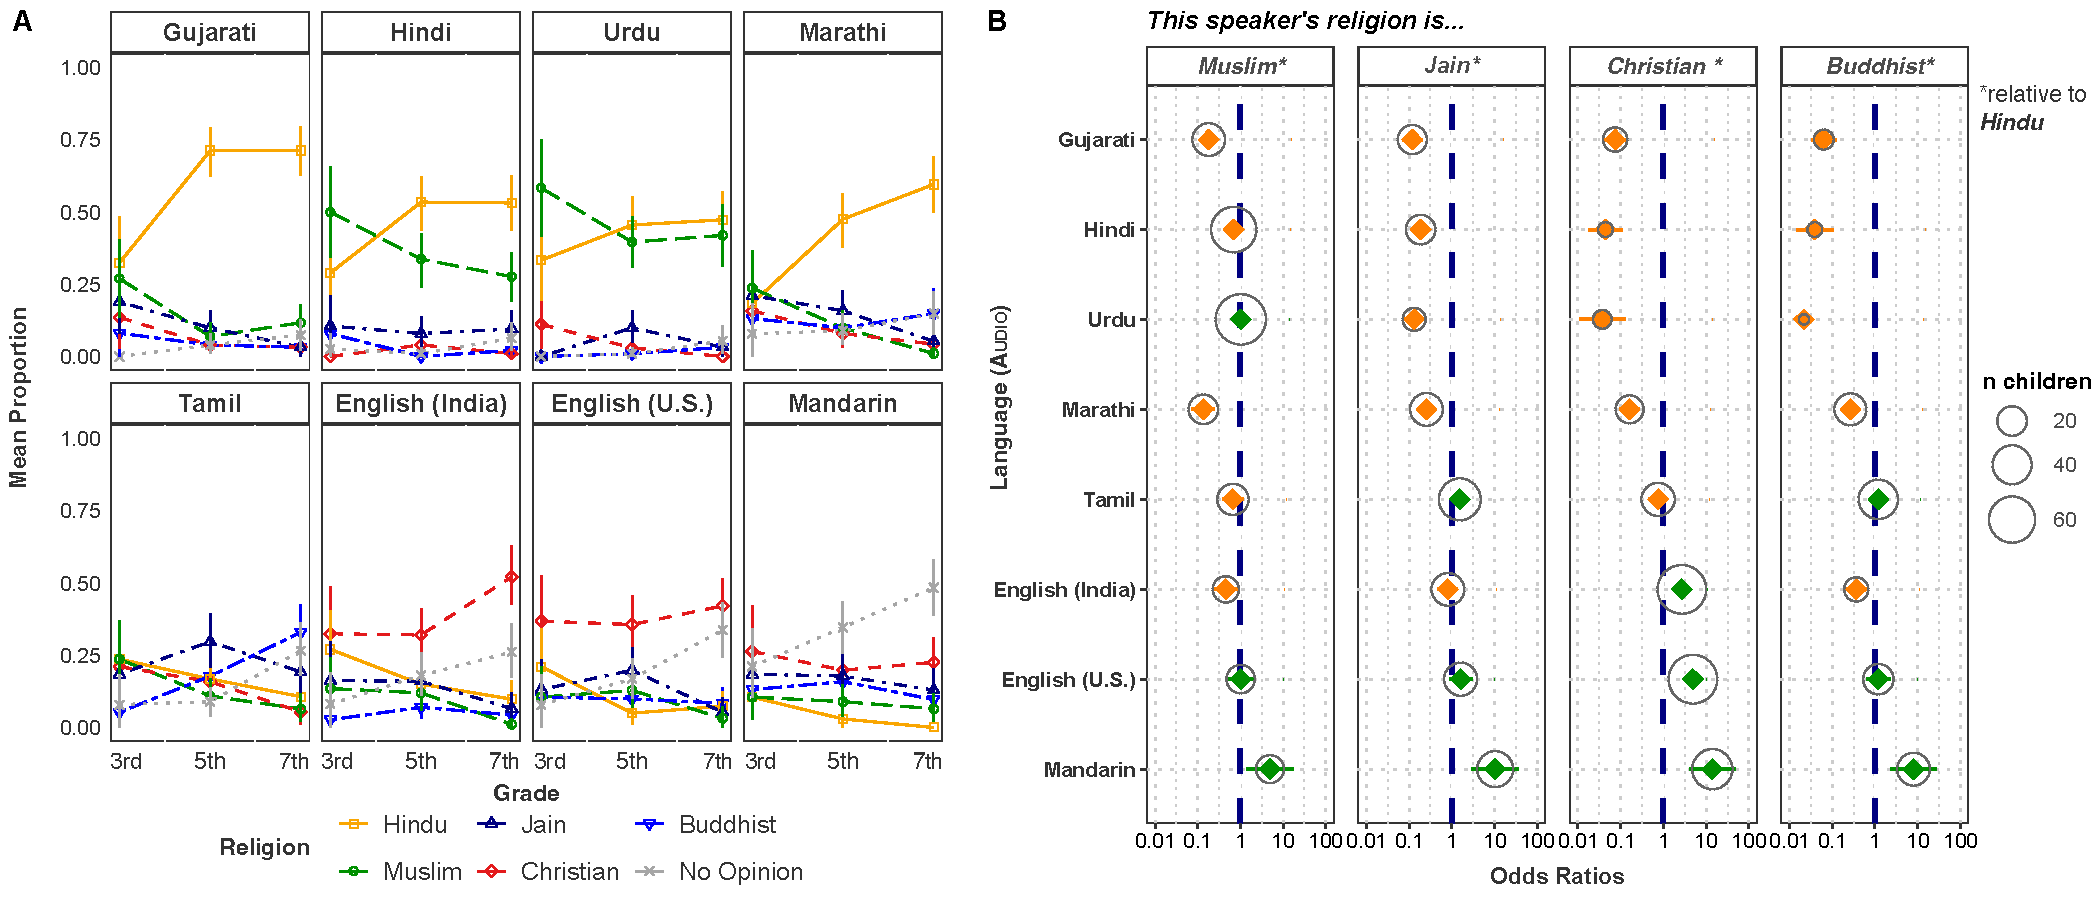
\includegraphics[width=\linewidth]{figures/combined_plots/combined_rel_finalized.pdf}
    \caption{\textit{Religious Association (``This speaker's religion is\ldots'') by Grade and Speaker Language.} 
    Points in \textbf{A} plot the proportion of trials on which each religion was selected at each grade (x-axis), for each language (panels), with error bars reflecting 95\% bootstrapped confidence intervals. 
    Points in \textbf{B} plot the estimates and 95\% bootstrapped confidence intervals for the odds ratios for selecting each religion (panels), relative to the reference option---``Hindu,'' given language (rows). 
    %each language in the comparison between the given categorical response (panels) and the reference group (Hindu), 
    Points are color-coded by the direction of the effect; points further from (and not intersecting with) the dashed vertical line at 1 represent greater differences between selections of that religion and selections of ``Hindu.'' 
    Bubble outlines reflect the number of children selecting each paneled religion for each language.} %that particular religion (panels) in response to that particular language (rows).
    \label{fig:religion}
\end{figure*}
\paragraph{Muslim (vs. Hindu).} 
Urdu was most strongly associated with Islam (the Urdu speaker was identified as ``Muslim'' on 42\% of trials). 
Relative to Hinduism, children were unlikely to identify speakers of Gujarati ($OR=0.18$ [$0.12$, $0.28$], $p<0.001$), Hindi ($OR=0.70$ [$0.51$, $0.96$], $p=0.027$), Indian English ($OR=0.46$ [$0.24$, $0.88$], $p=0.019$), and Marathi ($OR=0.14$ [$0.07$, $0.26$], $p<0.001$) as ``Muslim,'' and more likely to identify speakers of Mandarin as ``Muslim'' ($OR=4.97$ [$1.37$, $18.10$], $p=0.015$). 
Children tended to identify speakers of Mandarin as ``Muslim'' even more often, relative to ``Hindu,'' as they got older ($OR=2.71$ [$1.31$, $5.60$], $p=0.007$), and speakers of Gujarati ($OR=0.75$ [$0.57$, $0.98$], $p=0.035$) and Marathi ($OR=0.60$ [$0.38$, $0.95$], $p=0.028$) even less. %  (from 27\% of trials in 3$^{\textnormal{rd}}$ grade to 17\% of trials in 7$^{\textnormal{th}}$ grade).
The effects of child religion for the contrast between Muslim vs. Hindu religious associations differed across languages: on the one hand, both Hindu and Muslim participants were less likely to respond that Islam (relative to Hinduism) was the religion of the Marathi speakers (Hindu children: $OR=0.20$ [$0.12$, $0.35$], $p<0.001$; Muslim children: $OR=0.21$ [$0.25$, $0.91$], $p=0.037$). 
On the other hand, though both Hindu and Muslim children often inferred the Urdu speakers to be ``Muslim,'' they did so to reliably different degrees (23\% of Hindu child trials compared to 59\% of Muslim child trials), and Hindu children selected ``Muslim'' as the religion for Urdu speakers significantly less often than they selected ``Hindu'' (which they did on 63\% of trials; $OR=0.43$ [$0.28$, $0.66$], $p<0.001$). 
%The two groups' assumptions went in opposite directions for speakers of other languages.
For other languages, the two groups' assumptions went in opposite directions: for example, 
%For example, 
Muslim children predicted that the Gujarati speaker was Muslim on 20\% of trials (reliably more than they predicted the speaker was Hindu: $OR=3.29$ [$1.33$, $8.14$], $p=0.10$), while Hindu children almost never did (only 4\% of trials; $OR=0.09$ [$0.05$, $0.20$], $p<0.001$). 
Hindu children predicted that the Mandarin speakers were ``Muslim'' reliably more often than that they were ``Hindu'' (11\% of trials compared to $>1\%$; $OR=12.91$ [$1.68$, $98.96$], $p=0.014$), while Muslim children predicted the opposite ($OR=0.03$ [$0.00$, $0.33$], $p=0.005$).

\paragraph{Christian (vs. Hindu).}
Christianity was most often attributed to the speakers of both dialects of English (50\% of both Indian and U.S. English trials; reliably more often than Hinduism for Indian English: $OR=2.70$ [$1.76$, $4.13$]; U.S. English: $OR=4.92$ [$2.89$, $8.38$], $ps<0.001$), followed by Mandarin (36\% of trials; $OR=13.88$ [$4.02$, $47.87$], $p<0.001$). 
Christianity was almost never attributed to speakers of Gujarati, Hindi, Urdu, or Marathi ($2-9$\% of trials). 
It was selected reliably less often than Hinduism for Gujarati: $OR=0.07$ [$0.04$, $0.14$], Hindi: $OR=0.04$ [$0.02$, $0.11$], Urdu: $OR=0.04$ [$0.01$, $0.13$], and Marathi: $OR=0.16$ [$0.09$, $0.28$], $ps<0.001$). 
%Relative to Hinduism, children preferred Christianity as the religion of the Indian U.S. English 
With age, children became significantly more likely to assume that speakers of both Indian ($OR=2.42$ [$1.50$, $3.92$], $p<0.001$) and U.S. ($OR=2.38$ [$1.42$, $3.99$], $p<0.001$) English, as well as of Mandarin ($OR=3.50$ [$1.64$, $7.45$], $p<0.001$) were ``Christian,'' rather than ``Hindu,'' and even less likely to assume the same for speakers of Gujarati ($OR=0.63$ [$0.42$, $0.94$], $p=0.028$). These effects were generally carried by the Hindu children (Table~\religionchirelmodeltab); Muslim children exhibited a significant difference in their assumptions of Christianity vs. Hinduism only for Marathi-speakers (13\% vs. 28\% of trials, respectively; $OR=5.85$ [$1.11$, $30.92$], $p=0.037$). % from 31\% in 3$^{\textnormal{rd}}$ grade to 52\% in 7$^{\textnormal{th}}$) 
%and U.S. English ($OR=2.33$ [$1.36$, $3.99$]) % from 35\% in 3$^{\textnormal{rd}}$ grade to 43\% in 7$^{\textnormal{th}}$) 
%were Christian, rather than Hindu. 
% Marathi Muslim children more likely to think Christian, Hindu children less 

\paragraph{Jain (vs. Hindu).}
%Children became less likely to identify speakers as Jain with age ($OR=0.84$ [$0.76$, $0.92$]) %, from 15\% of 3$^{\textnormal{rd}}$ grade trials to 8\% in 7$^{\textnormal{th}}$ grade), 
Children selected ``Jain'' as the speaker's religion most often for speakers of Tamil, relative to other languages (24\% of trials), and became reliably more likely to say that speakers of Tamil were ``Jain,'' as opposed to Hindu, with age ($OR=1.89$ [$1.23$, $2.93$], $p=0.004$). 
They also reliably selected ``Jain,'' relative to ``Hindu'' for speakers of Mandarin ($OR=10.23$ [$2.93$, $35.65$], $p<0.001$), and did so more over time ($OR=3.51$; [$1.69$, $7.29$], $p<0.001$). 
Children were less likely to assume that speakers of Gujarati ($OR=0.12$ [$0.07$, $0.20$]), Hindi ($OR=0.19$ [$0.12$, $0.30$]), Urdu ($OR=0.13$ [$0.07$, $0.24$]), and Marathi ($OR=0.26$ [$0.16$, $0.41$], $ps<0.001$) were ``Jain'' over ``Hindu,'' and even less likely for Gujarati with age ($OR=0.59$ [$0.42$, $0.82$], $p=0.002$). 
The most striking differences between Hindu and Muslim children's patterns were in response to Marathi---where Hindu children were less likely to respond ``Jain'' relative to ``Hindu'' ($OR=0.08$ [$0.03$, $0.18$], $p<0.001$), while Muslim children did the opposite ($OR=5.86$ [$1.45$, $23.61$], $p=0.013$)---and in response to U.S. English, where Hindu children were more likely to respond ``Jain'' relative to ``Hindu'' ($3.02$ [$1.20$, $7.63$], $p=0.019$), while Muslim children did not show this pattern ($OR=0.16$ [$0.03$, $0.79$], $p=0.024$).

\paragraph{Buddhist (vs. Hindu).}
Buddhism was children's least frequent religious association (9\% of trials overall), and, like Christianity, was especially avoided for speakers of Gujarati (%5\% of trials; 
$OR=0.06$ [$0.03$, $0.13$]), Hindi ($OR=0.46$ [$0.01$, $0.11$]), %2\%; 
Urdu (%2\%; 
$OR=0.02$ [$0.00$, $0.11$]), and Marathi %12\%;
($OR=0.02$ [$0.00$, $0.11$], $ps<0.001$)---along with Indian English ($OR=0.37$ [$0.19$, $0.72$], $p=0.004$). %5\%
With age, children showed increases in their identification of speakers of Tamil ($OR=2.29$ [$1.35$, $3.88$], $p=0.002$), Mandarin ($OR=3.10$ [$1.41$, $6.82$], $p=0.005$), and U.S. English ($OR=2.01$ [$1.12$, $3.63$], $p=0.020$) as ``Buddhist'' ($ORs=1.85-2.59$), relative to as ``Hindu.'' 
Here again, effects were largely driven by the Hindu children. 
Hindu and Muslim children exhibited reliably different religious associations only with Marathi speakers: Muslim children associated the Marathi speaker with Buddhism on 20\% of Marathi trials ($OR=15.55$ [$2.73$, $88.76$], $p=0.002$) compared to just 3\% of Marathi trials for Hindu children ($OR=0.05$ [$0.02$, $0.14$], $p<0.001$). 

%Our analysis of children's inferences about each language speaker suggests that 
In sum, the particular religions children associated with familiar Indian languages were largely sensible: speakers of Gujarati and Marathi were generally assumed to be Hindu, and speakers of Hindi and Urdu were assumed to be Hindu or Muslim (with Hindu children being significantly less likely to identify Urdu speakers as Muslim). At the same time, children showed a surprising tendency to respond that Indian English speakers were Christian (on 52\% of trials in 7$^{\textnormal{th}}$ grade)---just as they did for speakers of U.S. English (on 42\% of trials in 7$^{\textnormal{th}}$ grade).  
With age, children generally avoided associating Tamil---a largely unfamiliar language to them---with Hinduism, instead associating it with Jainism or Buddhism.
In general, Hindu and Muslim children were more likely to identify a speaker as following their own religion. % own religion also influenced their responses, in that Hindu children were more likely in general to identify a speaker as Hindu, % (39\% of trials across standards, compared to 23\% of trials by Muslim children), In general, Muslim children tended to identify speakers as ``Muslim'' more often than Hindu children (22\% of trials, compared to 12\% of trials by Hindu children).
%and Muslim children were more likely in general to identify a speaker as Muslim. % (22\% of trials across standards, compared to 12\% of trials by Hindu children). 
This relative bias for the child's own religion was especially pronounced for the local language, Gujarati, where Hindu children identified the Gujarati speaker as Hindu on 73\% of trials across grades (compared to 57\% of trials by Muslim children), and Muslim children identified the Gujarati speaker as a Muslim on 18\% of trials across grades (compared to 7\% of trials by Hindu children), perhaps reflecting differences in these children's relative experience hearing Gujarati from Hindu versus Muslim speakers (e.g., due to residential segregation). 
\begin{figure*}
    \centering
    \includegraphics[width=\linewidth]{figures/combined_plots/combined_wealth_finalized.pdf}
    \caption{\textit{Wealth Association (``This speaker has\ldots'') by Grade and Speaker Language.}
    {In \textbf{A}, lines plot the mean predicted wealth, recoded on a scale from -1---``less money than the people in my city,'' to 1---``more money than the people in my city,'' for speakers of each language (panels), by children in each grade (x-axis). 
    %Error bars reflect 95\% bootstrapped confidence intervals. 
    In \textbf{B}, bars show the overall mean predicted wealth for speakers of each language. The dashed horizontal line marks the midpoint of the scale (``as much money as the people in my city''). 
    Error bars in \textbf{A} and \textbf{B} reflect 95\% bootstrapped confidence intervals.}}
    \label{fig:wealth}
\end{figure*}
\subsubsection{Wealth: This speaker has\ldots} 
All children selected a single response for each trial, and 61 children selected ``No opinion'' on at least one trial (265 trials total, including 49 in response to Mandarin, 45 in response to Marathi, and 39 in response to Tamil). 
Across languages and ages, children most often (39\% of trials) responded that the speaker had a comparable amount of wealth to the people in the child's city, followed by more (32\%) and less (15\%; see %Figure~\ref{fig:wealth} and 
Table~\wealthmeanstab).
Children reliably predicted greater wealth for speakers of both dialects of English (Indian: $OR=2.63$ [$1.78$, $3.88$]; U.S.: $OR=2.68$ [$1.82$, $3.93$]) and of Mandarin ($OR=3.46$ [$2.30$, $5.20$], $ps<0.001$; Table~\wealthmodeltab; Figure~\ref{fig:wealth}). 
As children got older, they became less likely to predict that speakers had more money ($OR=0.88$ [$0.79$, $0.98$], $p=0.018$; e.g., 3$^{\textnormal{rd}}$ to 7$^{\textnormal{th}}$ grade ``more money than the people in my city'' percentages by language: Gujarati: 39\% to 12\%, Hindi: 32\% to 12\%, Urdu: 31\% to 13\%, Marathi: 33\% to 12\%, Tamil: 37\% to 7\%, Indian English: 35\% to 34\%, U.S. English: 55\% to 27\%, Mandarin: 51\% to 34\%). 
By 7$^{\textnormal{th}}$ grade, children selected ``as much money as the people in my city'' on the plurality of trials regarding speakers of Gujarati (59\%), Hindi (58\%), Urdu (59\%), Marathi (44\%), Tamil (40\%), and U.S. English (40\%). 
Including an interaction between language and child age did not significantly improve model fit ($\chi^{2}(7)=8.03$, $p=0.33$).
%from 31--55\% of trials in 3$^{\textnormal{rd}}$ to 7--34\% of trials in 7$^{\textnormal{th}}$
%mean selection rates for each response by grade are plotted in Figure~\ref{fig:wealth}, and listed in Table~\wealthmeanstab). 

\subsection{Stereotypical Speaker Selection}
%Across all speaker-selection trials, the North Indian \textsc{Hindu} faces were the most frequently selected (23\% of all single-selection trials), making it the reference category. Below, we report results from models contrasting each other face with effects for the Hindu face, ordered
Model results for comparisons between the North Indian Hindu face (\textsc{Hindu}, the most frequent selection and reference category), and each of the other four faces appear below, ordered from the second-most frequently selected face to the least frequently selected one. 

\subsubsection{Languages Presented via Audio: \textit{Who could be speaking?}} 
Children across grades tended to select a single face in response to the speaker selection questions for languages presented via audio clips (91\% of trials overall). %95\% of trials in 3$^{\textnormal{rd}}$ grade, 89\% of trials in 5$^{\textnormal{th}}$ grade, and 90\% of trials in 7$^{\textnormal{th}}$ grade; ).  
Twenty-two children selected more than one face across 53 trials (including 10 for both Hindi and Urdu, and 7 for U.S English, Indian English, and Marathi) % 5 for Tamil, 4 for Gujarati, and 3 for Mandarin).
Children ($n=30$) selected ``No opinion'' on 39 trials (including 13 for Mandarin, 11 for Tamil, and 6 for Marathi). %, 3 for Gujarati and Urdu, 2 for U.S. English, and 1 for Hindi).
Figure~\ref{fig:faces-language-audio}A and Table~\faceaudiomeanstab\ show face selection means in response to each language presented auditorily, for each grade. A model with an interaction between language and child age resulted in a significantly better fit ($\chi^{2}(28)=184$, $p<0.001$). 
% Children selected the Hindu face as the speaker of Gujarati on the majority of trials (58\%)

\paragraph{South Indian Hindu faces {(D{\small{RAVIDIAN}} vs. H{\small{INDU}})}.} 
Children most often selected the South Indian \textsc{Dravidian} faces as speakers of Marathi audio clips (42\% of trials across ages). 
Compared to the North Indian \textsc{Hindu} faces, children were significantly less likely to select the \textsc{Dravidian} faces when hearing clips of Gujarati ($OR=0.49$ [$0.36$, $0.67$], $p<0.001$) and Hindi ($OR=0.53$ [$0.35$, $0.81$], $p=0.003$), and reliably more likely to select them when hearing clips of Indian English ($OR=2.85$ [$1.36$, $5.95$], $p=0.005$) or U.S. English ($OR=8.83$ [$2.91$, $26.77$], $p<0.001$). 
Children's odds of selecting the \textsc{Dravidian} over \textsc{Hindu} faces as speakers of Gujarati further decreased with age ($OR=0.81$ [$0.66$, $0.99$], $p=0.039$), but increased for Urdu clips ($OR=1.89$ [$1.34$, $2.65$], $p<0.001$). 

%%%%% BREAKDOWN OF N-1 RESPONSE CATEGORIES
\paragraph{White faces {(W{\small{HITE}} vs. H{\small{INDU}})}.}
Children were reliably more likely to select the \textsc{White} faces %over the \textsc{Hindu} faces 
as speakers of either English dialect (70\% of Indian English trials: $OR=16.57$ [$8.67$, $31.69$]; 66\% of U.S. English trials: $OR=40.19$ [$13.86$, $116.52$], $ps<0.001$), relative to the Hindu faces (4\% of Indian English trials; 2\% of U.S. English trials). 
Children rarely selected the \textsc{White} faces when presented with clips of Gujarati, Hindi, Urdu, or Marathi (4\%--7\% of trials) and were significantly less likely to select them relative to the \textsc{Hindu} faces as speakers of those languages (Gujarati: $OR=0.06$ [$0.03$, $0.14$]; Hindi: $OR=0.15$ [$0.07$, $0.32$]; Urdu: $OR=0.27$ [$0.13$, $0.57$]; Marathi: $OR=0.12$ [$0.05$, $0.25$], $ps<0.001$)---a tendency that increased with age for Gujarati ($OR=0.58$ [$0.37$, $0.92$], $p=0.020$). 
With age, children's odds of selecting the \textsc{White} relative to the \textsc{Hindu} faces significantly increased for Urdu ($OR=2.09$ [$1.09$, $3.99$], $p=0.026$), Indian English ($OR=2.05$ [$1.12$, $3.76$], $p=0.020$), U.S. English ($OR=2.58$ [$1.17$, $5.70$], $p=0.019$), and Mandarin ($OR=3.26$ [$1.66$, $6.40$], $p<0.001$).

\paragraph{Muslim faces {(M{\small{USLIM}} vs. H{\small{INDU}})}.} 
Children selected the \textsc{Muslim} faces most frequently when hearing audio clips of Urdu (53\%) and Hindi (48\%), and selected them reliably more often than the North Indian \textsc{Hindu} faces when hearing these languages (Urdu: $OR=3.67$ [$2.46$, $5.48$]; Hindi: $OR=1.78$ [$1.30$, $2.43$], $ps<0.001$). These effects increased with age (Urdu: $OR=3.59$ [$2.34$, $5.53$]; Hindi: $OR=2.80$ [$1.86$, $4.21$], $ps<0.001$), as did children's relative selection of the \textsc{Muslim} faces compared to the \textsc{Hindu} faces, in response to audio clips of Tamil ($OR=1.62$ [$1.02$, $2.57$], $p=0.042$), Indian English ($OR=2.97$ [$1.61$, $5.47$]), and Mandarin ($OR=4.04$ [$1.88$, $8.66$], $p<0.001$). 
Children were less likely to select \textsc{Muslim} faces, relative to \textsc{Hindu} faces, when hearing clips of Marathi ($OR=0.09$ [$0.04$, $0.22$]), and of Gujarati ($OR=0.11$ [$0.06$, $0.22$]---and even less likely as they got older: $OR=0.39$ [$0.28$, $0.56$], $ps<0.001$).

\paragraph{East Asian faces {(A{\small{SIAN}} vs. H{\small{INDU}})}.}
Children overwhelmingly selected the \textsc{Asian} faces as speakers of audio clips of Mandarin (74\% of trials, relative to 19\% of Tamil trials, 13\% of U.S. English trials, and 4\%--7\% of trials for all other languages). 
Children's odds of selecting the \textsc{Asian} face relative to the \textsc{Hindu} face were higher in response to clips of U.S. English ($OR=6.68$ [$2.15$, $20.79$], $p=0.001$) and Mandarin ($OR=21.12$ [$9.00$, $49.59$], $p<0.001$), but increased with age only for Mandarin clips ($OR=3.69$ [$2.01$, $6.77$], $p<0.001$). Children's odds were reliably lower in response to Gujarati ($OR=0.08$ [$0.04$, $0.16$], $p<0.001$), Hindi ($OR=0.18$ [$0.09$, $0.36$], $p<0.001$), Urdu ($OR=0.39$ [$0.20$, $0.77$], $p=0.006$), and Marathi ($OR=0.14$ [$0.07$, $0.26$], $p<0.001$), and further decreased for Gujarati in older children ($OR=0.63$ [$0.42$, $0.95$], $p=0.027$). 

\begin{figure*}
    \centering
    \includegraphics[width=\linewidth]{figures/combined_plots/combined_faces_audio_finalized.pdf}
    \caption{\textit{Mean Face Selection (``Who could be speaking?'') by Grade for Languages Presented Auditorily.} In \textbf{A}, points plot the proportion of trials on which each face was selected at each grade (x-axis) for each language (panels). 
    In \textbf{B}, points plot the odds ratios for each language (rows) in the multinomial mixed effects model predicting the selection of each face (panels) relative to the reference face---\textsc{Hindu}, color-coded by the direction of the effect. 
    The model included predictors whose effects are not plotted, i.e., for age and the interaction between language and age, along with random intercepts for child. 
    Bubble areas surrounding each point range reflect the number of children selecting that face for audio clips of that language.
    Error bars in \textbf{A} and \textbf{B} reflect 95\% bootstrapped confidence intervals.
    \label{fig:faces-language-audio}}
\end{figure*}

\subsubsection{Language Presented by Name: \textit{Who speaks [Language]?}}
In the block where languages were instead queried by name, 14 children selected more than one face (37 trials), and 14 children selected ``No opinion'' at least once (30 trials; including 14 for ``Gujarati''). %and 5 for Hindi, Urdu, Marathi, and Tamil). 
Mean rates of face selection for each language presented by name are plotted in Figure~\ref{fig:faces-language-name} and tabulated in Table~\facelabelmeanstab. 
A model with an interaction between language and child age resulted in a significantly better fit ($\chi^{2}(24)=133$, $p<0.001$). 
\begin{figure*}
    \centering
    \includegraphics[width=\linewidth]{figures/combined_plots/combined_faces_label_finalized.pdf}
    \caption{\textit{Mean Face Selection (``Who speaks \emph{[\textsc{Language}]}?'') by Grade for Languages Presented by Language Name.}  
    Points plot the proportion of trials for each language (panels) on which each face (lines) was selected at each grade (x-axis). %, with error bars reflecting 95\% bootstrapped confidence intervals. 
    In \textbf{B}, points plot the estimates for each language (in terms of odds ratios) in the multinomial mixed effects model described in the results, 
    predicting the selection of each face (panels) relative to the reference face---\textsc{Hindu}. %, including random intercepts for children, and age and the interaction between language and age as additional (not plotted) predictors. 
    Model-estimated effects are color-coded by direction; the areas of the surrounding bubbles reflect the number of children selecting that face as a speaker of that language. 
    Error bars in \textbf{A} and \textbf{B} reflect 95\% bootstrapped confidence intervals.}
    \label{fig:faces-language-name}
\end{figure*}
%%%%% BREAKDOWN OF N-1 RESPONSE CATEGORIES - FL
\paragraph{South Indian Hindu faces {(D{\small{RAVIDIAN}} vs. H{\small{INDU}})}.} 
Children generally selected the \textsc{Dravidian} faces as speakers of ``Tamil'' (54\% of ``Tamil'' trials) and ``Marathi'' (38\% of trials), and mostly avoided them when asked who speaks ``English'' (2\% of trials). 
Children selected \textsc{Dravidian} faces, reliably more often than the North Indian \textsc{Hindu} faces, as speakers of ``Tamil'' ($OR=2.11$ [$1.54, 2.89]$, $p<0.001$), a tendency which increased with age (from 33\% of trials in 3$^{\textnormal{rd}}$ grade to 68\% of trials in 7$^{\textnormal{th}}$ grade; $OR=1.46$ [$1.10, 1.94]$, $p=0.009$). Children were significantly less likely to choose the \textsc{Dravidian} faces, relative to the \textsc{Hindu} faces, as speakers of ``Gujarati'' ($OR=0.35$ [$0.25$, $0.49$]) or ``Hindi'' ($OR=0.27$ [$0.17$, $0.45$], $ps<0.001$).

\paragraph{White faces {(W{\small{HITE}} vs. H{\small{INDU}})}.}

Children showed a strong selective association between English and the \textsc{White} faces, selecting them on 85\% of all trials asking about ``English'' (and reliably more often than the \textsc{Hindu} faces, selected on just 2\% of ``English'' trials: $OR=67.11$ [$21.12$, $213.22$]), but on just 2\%--9\% of trials querying any other language (Gujarati: $OR=0.02$ [$0.01$, $0.09$], $p<0.001$; Hindi: $OR=0.05$ [$0.02$, $0.18$], $p<0.001$; Urdu: $OR=0.05$ [$0.00$, $0.90$], $p=0.042$; Marathi: $OR=0.12$ [$0.07$, $0.22$], $p<0.001$; Tamil: $OR=0.35$ [$0.21$, $0.59$], $p<0.001$). 
The \textsc{White} faces were also selected reliably more often than the North Indian \textsc{Hindu} faces as speakers of ``Chinese'' ($OR=4.46$ [$1.12$, $17.57$], $p=0.034$; 8\% vs. 2\% of ``Chinese'' trials). 
With age, children became even less likely to select the \textsc{White} faces as speakers of ``Gujarati'' (from 6\% of trials in 3$^{\textnormal{rd}}$ grade down to 1\% in 7$^{\textnormal{th}}$ grade; $OR=0.47$ [$0.24, 0.90]$, $p=0.023$).

\paragraph{Muslim faces {(M{\small{USLIM}} vs. H{\small{INDU}})}.} 
Children most often selected these faces as speakers of ``Urdu,'' which they did significantly more often than the North Indian \textsc{Hindu} faces ($OR=12.57$ [$6.98$, $22.61$]), and even more with age ($OR=2.18$ [$1.41$, $3.37$], $ps<0.001$; from 58\% of trials in 3$^{\textnormal{rd}}$ grade to 93\% of trials in 7$^{\textnormal{th}}$). 
%Relative to the North Indian \textsc{Hindu} faces, children reliably ($OR=12.44$ [$6.91$, $22.37$])---and increasingly with age ($OR=2.15$ [$1.39$, $3.34$])---identified the \textsc{Muslim} faces as potential speakers of ``Urdu'' (doing so on 58\% of trials in 3$^{\textnormal{rd}}$ grade and 93\% of trials in 7$^{\textnormal{th}}$). 
Children were also significantly more likely to select the \textsc{Muslim} faces, relative to the \textsc{Hindu} faces, as speakers of ``Hindi'' ($OR=1.57$ [$1.18$, $2.10$], $p=0.002$), and significantly less likely to select the \textsc{Muslim} faces as speakers of the other regional Indian languages: ``Gujarati'' ($OR=0.16$ [$0.10$, $0.25$]), ``Marathi'' ($OR=0.03$ [$0.01$, $0.10$]), and ``Tamil'' ($OR=0.11$ [$0.05$, $0.27$], $ps<0.001$).

\paragraph{East Asian faces {(A{\small{SIAN}} vs. H{\small{INDU}})}.}
Children were most likely to select the \textsc{Asian} faces when asked who speaks ``Chinese'' (86\% of all ``Chinese'' trials), and  selected them reliably more often than the North Indian \textsc{Hindu} faces ($OR=67.89$ [$19.11$, $241.16$], $p<0.001$). 
Children's odds of selecting the \textsc{Asian} relative to the \textsc{Hindu} faces were also significantly greater when asked to identify speakers of ``English'' ($OR=5.25$ [$1.50$, $18.39$]), though the difference in selection rates was only between 9\% vs. 2\% of ``English'' trials. 
Children's odds of selecting the \textsc{Asian} face were significantly lower than those of selecting the \textsc{Hindu} face for all other languages except Urdu (``Gujarati:'' $OR=0.05$ [$0.02$, $0.12$]; ``Hindi:'' $OR=0.10$ [$0.05$, $0.22$]; ``Marathi:'' $OR=0.07$ [$0.03$, $0.15$]; ``Tamil:'' $OR=0.25$ [$0.13$, $0.46$], $ps<0.001$), and showed further decreases with age for ``Gujarati,'' specifically ($OR=0.60$ [$0.37$, $0.95$], $p=0.031$---from 10\% of ``Gujarati'' trials in 3$^{\textnormal{rd}}$ grade to 1\% of trials in 7$^{\textnormal{th}}$). 
%more likely to identify the \textsc{asian} face as a speaker of Chinese (from 73\% in 3$^{\textnormal{rd}}$ grade to 96\% in 7$^{\textnormal{th}}$). \famodtab
\begin{figure*}
    \centering
    \includegraphics[width=\linewidth]{figures/combined_plots/combined_learning_finalized2.pdf}
    \caption{\textit{Normalized Learning Predictions for Each Face, by Language.} \textbf{A} shows the mean learning---on a scale from 1=``0\% (Not at all)'' to 3=``100\% (Very well)''---predicted for each category of face (lines) by children in each grade (x-axis). 
    In \textbf{B}, diverging bars reflect the number of children predicting below- (grey) versus above- (colored) average learning for the individuals represented by each face category, normalized by language (panels). 
    All error bars plot 95\% bootstrapped confidence intervals. 
    \label{fig:faces-learning-diverging}}
\end{figure*}
\subsection{Presentation Modality}
To directly test the effects of presentation modality on children's speaker selections, we fit an additional model to children's face selection data in response to all languages except English, with age, language, presentation modality (\textit{audio} or \textit{name}), the interaction of language and modality, and random intercepts for each child. The interaction between language and modality was significant ($\chi^2(20)=957$, $p<0.001$), and suggested an amplification of the selective relations between languages and faces for the same language when it was presented by name, rather than via audio clip (see Table~\facemodalitytab; Figure \nonengbarplot).

An additional model of face selections for the three trial types querying English (\textit{Indian English Audio}, \textit{U.S. English Audio}, and \textit{``English'' Name}) showed that children responded similarly across English trials, regardless of the dialect of English or how it was presented (Table~\faceenglishmodalitytab, Figure~\engbarplot). 
That is, across English trial types, children typically selected the \textsc{Hindu} face less often than any of the other faces, regardless of whether they were hearing audio clips of Indian or U.S. English, or being asked about speakers of ``English'' by name. 
More specifically, children reliably selected the \textsc{White} more than the \textsc{Hindu} face for all three trial types (``English'' by name: $OR=67.99$ [21.61, 213.91]; Indian English audio: $OR=38.71$ [14.31, 104.72]; U.S. English audio: $OR=14.91$ [8.06, 27.60], $ps<0.001$). 
When asked who ''could be speaking English'' children also selected both the \textsc{Muslim} ($OR=4.33$ [$1.23$, $15.25$], $p<0.001$) and \textsc{Asian} ($OR=4.77$ [$1.37$, $16.59$], $p=0.014$) faces reliably more often than the \textsc{Hindu} faces. 
They also selected the \textsc{Dravidian} ($OR=8.41$ [$2.98$, $23.78$]) and \textsc{Asian} ($OR=6.92$ [$2.42$, $19.80$], $ps<0.001$) faces reliably more often than the \textsc{Hindu} faces in response to audio clips of Indian English, and they  selected the \textsc{Dravidian} faces reliably more often than the \textsc{Hindu} faces in response to audio clips of U.S. English ($OR=2.70$ [$1.34$, $5.41$], $p=0.005$).

In sum, selective face associations tended to become more conventionalized with age for both auditorily presented and named languages (a greater proportion of children chose the same face(s) as speakers of a given audio clip, or for a given named language). 
Gujarati was generally paired with the \textsc{Hindu} faces, Hindi was paired with the \textsc{Hindu} and \textsc{Muslim} faces,  Urdu was paired with the \textsc{Muslim} faces,  Marathi with the \textsc{Hindu} and \textsc{Dravidian} faces, Tamil with the \textsc{Dravidian} faces, English  with the \textsc{White} faces (for \textit{both} Indian and U.S. dialects in the audio task), and Mandarin with the \textsc{Asian} faces. 
These associations were generally more robust when children were queried by language name, suggesting a role for the cultural transmission of associations between languages and ethnic, religious, and regional social groups. 

\subsection{Linguistic Essentialism: \textit{How well will they come to learn\ldots}} 
Finally, we explored children's tendency to essentialize language via their intuitions of how well each of five languages (``Gujarati,'' ``Hindi,'' ``Tamil,'' ``English,'' and ``Chinese'') would be learned by each speaker, under identical learning conditions  
%\textcolor{red}{low Cronbach's alpha for 3 questions targeting essentialism, so not analyzed as a construct}
%We fit mixed effects linear models to children's learning ratings (1--3) for each face individually, with language and child age as predictors, random intercepts for individual children, and the interaction between language and child age when its inclusion improved model fit 
(see Table~\learningmeanstab\ for mean estimated learning success for each face by grade and Figure~\ref{fig:faces-learning-diverging} for relative normalized learning ratings by face). 
Significant results from ordinal mixed effects models fit separately to the data for each language (Tables~\learningmodeltabs) are described below. 

\paragraph{``\textit{Gujarati}?''}
Compared to the people represented by the \textsc{Hindu} faces, children predicted significantly worse learning of ``Gujarati'' by the naive learners represented by the \textsc{Muslim} ($OR=0.22$ [$0.12$, $0.40$]), \textsc{Dravidian} ($OR=0.08$ [$0.04$, $0.15$]), \textsc{White} ($OR=0.04$ [$0.02$, $0.07$]), and \textsc{Asian} ($OR=0.02$ [$0.01$, $0.03$]) faces ($ps<0.001$). 
There was a significant interaction between language and child age ($\chi^{2}(4)=12.3$, $p=0.015$), such that older children's ``Gujarati'' learning predictions for the people represented by \textsc{White} faces were even lower than younger children's ($OR=0.60$ [$0.41$, $0.87$], $p=0.007$). 

\paragraph{``\textit{Hindi}?''}
Compared to the \textsc{Hindu} learners, children predicted significantly worse learning of ``Hindi'' by the individuals represented by the \textsc{Dravidian} ($OR=0.32$ [$0.18$, $0.57$]), \textsc{White} ($OR=0.09$ [$0.05$, $0.17$]), and \textsc{Asian} ($OR=0.05$ [$0.03$, $0.10$]) faces ($ps<0.001$). 
There was a significant interaction between language and child age ($\chi^{2}(4)=10.9$, $p=0.027$), such that older children predicted even worse learning by the people represented by the \textsc{White} faces, relative to the people represented by the \textsc{Hindu} faces ($OR=0.63$ [$0.44$, $0.90$], $p=0.011$). 

\paragraph{``\textit{Tamil}?''}
Children predicted significantly worse learning of ``Tamil'' by the individuals represented by the \textsc{Muslim} ($OR=0.29$ [$0.17$, $0.50$], $p<0.001$), \textsc{White} ($OR=0.35$ [$0.21$,  $0.60$], $p<0.001$), and \textsc{Asian} ($OR=0.40$ [$0.23$, $0.70$], $p=0.001$) faces, relative to the \textsc{Hindu} faces, and significantly better learning of ``Tamil'' by the individuals represented by the \textsc{Dravidian} ($OR=2.10$ [$1.19$, $3.71$], $p<0.001$) faces. There was a significant interaction between language and child age ($\chi^{2}(4)=23.7$, $p<0.001$), such that, with age, children predicted even better ``Tamil''-learning by the learners represented by the \textsc{Dravidian} faces ($OR=1.52$ [$1.03$, $2.25$], $p=0.034$), and even worse ``Tamil''-learning by those represented by the \textsc{White} faces ($OR=0.70$ [$0.50$, $0.99$], $p=0.045$). 
\begin{figure*}
    \centering
    \includegraphics[width=.7\textwidth]{figures/std_plots/id_accuracy_std.pdf}
    \caption{\textit{Language Identification Accuracy by Grade.} Points plot mean accuracy by grade (x-axis), color-coded by language (lines), with error bars representing 95\% bootstrapped confidence intervals.}
    \label{fig:lang-id-by-std}
\end{figure*}
\paragraph{``\textit{English}?''}
Children predicted significantly better ``English''-learning by the individuals represented by the \textsc{White} ($OR=18.55$ [$9.71$, $35.41$], $p<0.001$) and \textsc{Asian} ($OR=2.20$ [$1.26$, $3.85$], $p=0.006$) faces, relative to the \textsc{Hindu} faces. An interaction between language and child age significantly improved model fit ($\chi^{2}(4)=11.5$, $p=0.022$), suggesting that the relative effects of language were different for older versus younger children, though none of these achieved significance.

\paragraph{``\textit{Chinese}?''}
Compared to the learners represented by the \textsc{Hindu} faces, children predicted significantly better learning of ``Chinese'' by the people represented by the \textsc{White} ($OR=2.16$ [$1.24$, $3.77$], $p=0.006$) and \textsc{Asian} ($OR=146.96$ [$58.95$, $366.33$], $p<0.001$) faces, and significantly worse learning by the individuals represented by the \textsc{Dravidian} faces ($OR=0.52$ [$0.29$, $0.93$]). An interaction between language and child age did not improve model fit ($\chi^{2}(4)=4.07$, $p=0.4$).

In sum, children predicted that individuals of some ethnicities and religions would be better at learning particular languages, and these predictions often grew stronger with age. %predictions of different individuals' language-learning capacity differed by their ethnic/religious identity, and often showed greater divergence across faces with age. (e.g., children became \textit{more}, not less, likely to predict greater learning...)
\subsection{Language Identification}
% Significant results from logistic regression: 
%[Gujarati]	5.31 ***	3.26 – 9.40	<0.001
%[Hindi]	7.52 ***	4.49 – 13.75	<0.001
%[Urdu]	0.09 ***	0.04 – 0.17	<0.001
%[Tamil]	0.50 ***	0.34 – 0.72	<0.001
%[English(India) 2.22 ***	1.54 – 3.28	<0.001
%[English (U.S.)]	18.03 ***	8.93 – 44.50	<0.001
%[Mandarin]	1.78 **	1.23 – 2.61	0.003
%[Gujarati] child age centered	1.68 **	1.25 – 2.34	0.001
%[Urdu] × childage centered	0.37 ***	0.22 – 0.60	<0.001
%[Tamil] × childage centered	0.52 ***	0.35 – 0.76	0.001
Mean accuracy by language and grade are plotted in Figure~\ref{fig:lang-id-by-std}. 
Children became more accurate at identifying the audio clips with age (e.g., 50\% overall accuracy in 3$^{\textnormal{rd}}$ grade and 68\% accuracy in 7$^{\textnormal{th}}$ grade). Children struggled most with identifying Urdu ($M=0.11$ [$0.05, 0.17]$), Tamil ($M=0.33$ [$0.25, 0.41]$), and Marathi ($M=0.59$ [$0.51, 0.68]$). 
Interestingly, children showed selective associations with languages---the same ones that would become the most common associations in 7$^{\textnormal{th}}$ grade---even when they could not actually identify the language. 
For example, 3$^{\textnormal{rd}}$-graders who were unable to name Urdu still selected the \textsc{Muslim} faces as the speakers for the Urdu audio clips and ``Muslim'' as the Urdu-speakers' religion on 45\% of trials, and Gujarat as the speaker's geographic origin on 70\% of trials. 
Similarly, 3$^{\textnormal{rd}}$-graders who failed to identify Mandarin Chinese still selected the \textsc{Asian} faces for the Mandarin audio clips on 46\% of trials. %, and identified the Mandarin speaker as ``foreign'' on 25\% of trials. 
And 3$^{\textnormal{rd}}$-graders who were unable to identify Tamil or Marathi nonetheless recognized their speakers as likely ``from another place in India'' (48\% of trials by children who couldn't identify Tamil, and 31\% of trials by children who couldn't identify Marathi).  %45% Urdu-muslim, 15\% Marathi-Hindu
% Marathi-hindu face 24%  (only in those who got Marathi id wrong)
% Tamil-dravidian 12%
% Tamil-different state 48%
% Marathi-different state 31%
% Children were 
%own subsection for familiarity analyses
% Geographic origin --- went in opposite directions
% Religious 

\subsection{Language Familiarity}
To directly assess the effect of children's recognition and familiarity with each language, we used children's self-reported language backgrounds and their accuracy on the language identification task to form a new composite variable for language \textit{familiarity}. 
A language was coded as ``familiar'' for a given child if they either listed it as a language they knew or if they correctly named it when played an audio clip in the \textit{Language Identification} block. %As this was an English-medium school, it is maybe unsurprising that children
We updated the multinomial models reported in each section to include an interaction between language %(excluding Hindi and Indian English, for which there was insufficient variance) 
and familiarity %this new composite familiarity variable 
in predicting each set of categorical responses. %, relative to the reference response. 
Models for all question blocks of this type (geographic origin and religious associations, speaker selections) %except speaker wealth associations 
showed a significant interaction between language and familiarity, suggesting that children's degree of familiarity with each language influenced their associations with its speakers. 
%To further interrogate these effects, we 
%While full model details appear in the supplement, we highlight here...
%Whether or not children were familiar with the language did not significantly influence their estimates of its speakers' wealth (see Table~\wealthfamiliartab).
%Significant effects comparing the Muslim to the Hindu faces for children based on familiarity with each language were in the same direction when responding to clips of all languages but Marathi and Tamil, where children who neither listed nor recognized these languages were  less likely to select the Muslim face, while children who did were more likely to select the Muslim face. 
%In our complementary model including participants' language familiarity, 
%For example, while children coded as `unfamiliar' with Urdu were unlikely to identify its speakers as from ``another place in India'' ($OR=0.06$ [$0.02$, $0.13$]), those familiar with Urdu reliably did ($OR=24.01$ [$2.29$, $252.16$]). 
For example, children's odds of selecting a South Indian \textsc{Dravidian} face over a North Indian \textsc{Hindu} face as a potential speaker of the Tamil audio clips were significantly higher among children familiar with Tamil ($n=45$; %who either listed Tamil as a language they had experience with and/or who were able to correctly label an audio clip as containing ``Tamil'' 
$OR=2.58$ [$1.52$, $4.38$], $p<0.001$). 
Similarly, children who were able to correctly label the Mandarin clip ($n=81$; no child reported expressive or receptive knowledge of Mandarin) showed an even greater tendency to select the \textsc{Asian} over the \textsc{Hindu} faces as speakers of the Mandarin clips ($OR=32.01$ [$7.46$, $137.34$], $p<0.001$), compared to children ($n=47$) who failed to correctly identify it ($OR=4.85$ [$1.99$, $11.80$], $p=0.001$). 
%For example, while even children who did not correctly identify Mandarin Chinese nonetheless selected both alternate options over Gujarat, the effect was much greater in the children who had correctly identified it by audio. Similar for Marathi.
\section{General Discussion}

Despite the prevalence of multilingualism globally, most research on sociolinguistic development has focused on monolingual children in environments with relatively little linguistic diversity, and, as such, has not systematically addressed what children take different languages to socially signify. 
The present study aimed to fill this gap by tracing the development of social inferences and essentialist beliefs about languages among multilingual children and adolescents in Gujarat, India. 
Although multilingual experience could in principle make children less likely to make stereotyping inferences about speakers of a language---as multilingual children might expect an individual to know languages beyond the one they are currently using---we were interested in whether children in our sample might nevertheless exhibit social associations with different languages across a variety of dimensions. To examine this possibility, we presented children with unlabeled audio clips of eight different languages or dialects and probed associations with speakers' geographic origin, religion, wealth, and facial appearance (while also probing the latter using only language names). 
We also measured essentialist beliefs about language by asking children whether individuals of different ethnic or religious identities would vary in their ability to learn different languages if they had no prior experience with them.

Children in our sample selectively linked the different languages we presented with the different social dimensions we probed, and these patterns generally became more reliable with age. %Specifically, w
With respect to geographic origin, with age, children progressively identified speakers of audio clips of Gujarati as being from Gujarat while often judging speakers of the Marathi and Tamil clips as originating from ``another part of India'' and judging speakers of the U.S. English, Mandarin and Indian English clips as originating from ``outside India.'' 
With respect to religion, children often assumed that speakers of the Gujarati and Marathi clips were Hindu. With age, they progressively inferred that speakers of the Urdu clips were Muslim, and that speakers of the U.S. and Indian English clips were Christian. 
(Interestingly, Hindu and Muslim children were also in general more likely to identify speakers as following their own religions). 
With respect to wealth, children predicted that speakers of Mandarin and of either dialect of English had more money than they did, while generally becoming less likely with age to say that speakers of other languages had more money than they did. 
Finally, with age, children also selectively linked languages with faces that stereotypically corresponded to different ethnic or religious identities, for example pairing speakers of Gujarati with North Indian faces, Urdu with Muslim faces, Mandarin with East Asian faces, Tamil with Dravidian faces, and U.S. and Indian English with white faces; interestingly, our analyses found that these tendencies were often reliably more pronounced when facial associations were probed with language names (e.g., ``Who is speaking \textit{English}?'') compared to via audio clips alone. Children also appeared to understand these associations in an essentialist manner, predicting increasingly with age that individuals of some ethnicities and religions would be better at learning particular languages. 
 % (e.g., judging that a White person would be better able to learn English than individuals of other ethnic groups, even when told that none of these individuals had any prior experience with English). 

%Perhaps because most prior work in sociolinguistic development has been conducted with monolingual children with relatively little multilingual experience, 
Studies of sociolinguistic development have typically assessed children's social associations with a small number of varieties of the same language \parencite[e.g.,][]{weatherhead2019preschoolers, mccullough2019regional,kinzler2013northern} or else contrasted associations with children's own language versus a single, unfamiliar language \parencite[e.g.,][]{liberman2017preverbal, hirschfeld1997young, kinzler2012children, kinzler2007native, moon1993two}. Our findings extend this prior work in suggesting that---when faced with significant linguistic and social variability---children nevertheless attribute social information to languages in systematic and nuanced ways. 
Notably, the sociolinguistic associations that children in our sample exhibited could not be explained by a simple tendency to judge that people who spoke different languages from children's own would be different from them \parencite{hirschfeld1997young}. 
Such a heuristic would have predicted largely similar judgments regarding the multiple languages that individual participants did not speak (e.g., making similar judgments about Tamil, Urdu, Marathi, and Mandarin, which were unfamiliar to many of our participants). 
This is not what we saw.\footnote{One example of a case in which children may have used a ``different language = different from me'' strategy was in their judgments of the religion of Tamil speakers. With age, children were more likely to identify Tamil speakers as Jain or Buddhist, an association that is unconnected to actual fact. Tamil was unfamiliar to many of our participants, and lacking any evidence about the religion of speakers of these languages, children may have guessed that they also practiced an unfamiliar religion.} 
Relatedly, children's responses could not be explained by a general tendency to project positive traits onto individuals who spoke the same languages they did (e.g., judging those speakers as nicer or smarter; \cite{santhanagopalan2021nationality}), given that some of the dimensions that we probed---including facial appearance, geographic origin, and religion---are not easily organized along a positive--negative continuum.

Instead, children in our sample developed specific sociolinguistic associations, which often reflected regularities in the real world: e.g., Tamil and Marathi \textit{are} languages that derive from other regions of India (outside of Gujarat), Urdu speakers \textit{do} tend to be Muslim, Tamil speakers \textit{do} tend to look Dravidian, and U.S. English speakers \textit{do} tend to have more wealth than many people who live in Gujarat, due to global wealth inequalities. 
(One striking exception to this pattern of providing veridical associations were children's judgments of speakers of Indian English, which we return to below). 

Our findings provide preliminary evidence that children in our sample may have constructed these and other associations both by attending to ``bottom-up'' correlations in their real-world environmental experience (e.g., hearing a language spoken and attending to characteristics of the speakers), but also via ``top-down'' transmission of information about speakers of different languages (e.g., messages about a language and its speakers). 
Attesting to the role of bottom-up experience, even children who could not identify the language audio clips nevertheless exhibited systematic associations with those clips (e.g., linking Mandarin clips with East Asian faces). %And speaking to the role of higher-level conceptual knowledge, recall that 
Children were also more systematic in linking different languages with stereotypical faces when these associations were probed via language name (e.g., ``Who speaks \textit{Urdu}?''), compared to when they were probed with unlabeled audio clips. This latter pattern of findings suggests that children's associations between languages and ethnic or religious identity were partly linked to higher-level conceptual knowledge about those languages (e.g., that speakers of ``Urdu'' tend to be Muslim), such that this knowledge could be cued by language names without necessarily being accessible from listening to audio clips of Urdu being spoken. 
More generally, we found that children who had some degree of familiarity with each language---as indexed by children either listing the language as one they had experience with or correctly naming it when presented an audio clip---were more likely to exhibit the systematic social associations we measured (e.g., about speakers' geographic origin, religion, etc.), suggesting an important role for both bottom-up and top-down experience.  %(e.g., for children who did not recognize an audio clip as containing ``Urdu''). %It will be important to explore the interplay of bottom-up and top-down processes in the development of sociolinguistic associations in future work.

Based on the intuition that a multilingual child in a multilingual context might assume that other people will know multiple languages, our findings present a puzzle: Why were children in our sample so willing to make social inferences about a speaker based on the language they were using when they could easily have assumed that the speaker knew other languages, as well? One intriguing possibility is that children's responses did not reflect their beliefs about actual real-world speakers, \textit{per se}, but instead their understanding of the different, idealized \textit{personae} that a speaker can embody and project when they use different languages.  
Sociolinguistic theory defines \textit{personae} as ``\ldots holistic, ideological social types that are recognizably linked with ways of being and speaking'' (\cite{donofrio2020personae}, p. 1; see also \cite{d2016social}), and has used this construct to characterize the social identities associated with styles within a language that speakers draw upon: e.g., an English speaker can perform shallowness by using features of the ``Valley Girl'' style \parencite[e.g., including uptalk and using `like' as a discourse marker;][]{pratt2017jaw, d2015persona}. We suggest that this construct can be fruitfully extended to characterize how people make sense of the social meaning of different languages within multilingual contexts: e.g., such that, for children in our sample, the use of Gujarati evokes a local, Hindu, and North Indian persona, the use of English evokes a foreign, wealthy, white, and Christian persona, and so on. 

This proposal may help make sense of a striking pattern of findings we observed when probing children's judgments of speakers of Indian English audio clips. Children generally judged these speakers similarly to speakers of American English clips---as white, originating from outside of India, and Christian. Moreover, these surprising tendencies often became more---rather than less---pronounced with age. %\footnote{The exception to this generalization is children's attributions of greater relative wealth to the speakers of Indian English, which did not become particularly more pronounced with age.} 
These findings are unexpected if we take children's responses to reflect their beliefs about the actual characteristics of speakers in their real-world environment, given that our participants were students at an English-medium school who heard ample Indian English spoken by teachers, staff, and peers from their community---who were themselves rarely Christian and never white. Instead, we suggest that, for children in our sample, the use of Indian English evokes an idealized persona that is foreign, Christian, and white, which may itself be shaped by beliefs about and associations with speakers of British and American English. %(for which these associations have more basis in fact). 
Understanding the role of personae in children's developing sociolinguistic competence will be an important direction for future work.

A final striking finding that emerged from our study was that children exhibited essentialist beliefs about language learning---e.g., judging that, compared to individuals of other ethnicities, and even if they had no prior experience with the language, a white person would be better able to learn English, a North Indian person would be better able to learn Hindi and Gujarati, an East Asian person would be better able to learn Chinese, and so on. Such responses typically became more pronounced with age, which stands in contrast to prior work suggesting that essentialism of language decreases after the preschool years \parencite{kinzler2012children} and is diminished among bilingual children \parencite{byers2015bilingualism, dautel2018once}. Yet it is important to note that these prior studies employed different measures of essentialism than we did here (see Methods section), asking whether children and adults view language as biologically- or culturally-transmitted (e.g., via switched-at-birth paradigms; \cite{hirschfeld1997young, sun2023essentialist, byers2015bilingualism}), or by evaluating the stability of language relative to race over the lifespan (e.g., by asking whether a child who was white and spoke English would be more likely to change their language or race as an adult; \cite{kinzler2012children, dautel2018once}). Thus, future work is needed to address how our measure of linguistic essentialism correlates with previously-used measures, and whether it taps into the same underlying construct. Still, our results raise the intriguing possibility that language learning ability is particularly likely to be essentialized for individuals who experience the difficulty of trying to learn a new language later in life (as was the case for many of our participants, who were non-native learners of English), since this difficulty could lead individuals to assume that those who speak other languages fluently possess an innate, biological advantage for learning those languages. Future work could test this idea by assessing potential differences in older children's propensity to essentialize the learning of a specific language---particularly a language that is strongly correlated with an ethnicity to which the child does not belong---as a function of whether the children themselves are engaged in learning that language in their school or not. %More generally, it will be interesting in future work to explore how different facets of linguistic essentialism emerge and change across the lifespan, and how this might be shaped by multilingual experience.

\subsection{Future Directions and Conclusion}
The present study raises a number of questions for future research. To begin, although our findings provide an example of how children can selectively link the use of different languages with different social dimensions, our conclusions should of course not be generalized beyond the sample and context we studied. It will be valuable to understand similarities and differences in how children in other developmental contexts might ascribe social significance to the use of different languages in their respective environments. For example, the present study focused on dimensions that were relevant to understanding linguistic variation in the context we studied (e.g., region of origin, religion), but it is likely that children in other contexts will invoke other dimensions to understand the linguistic variation in their specific environments (e.g., caste, majority/minority status). Future work could further characterize how such sociolinguistic associations arise over development and explore how these associations are constructed (e.g., via direct multilingual experience, testimony from others, etc.).

Importantly, we note that although our work focused on the social information that children ascribe to a person who is using a single, specific language, it is likely that children in multilingual contexts expect individuals to know multiple languages beyond the one they are currently using. Thus, it will be interesting to explore how children understand speakers who use different intersections of languages (e.g., a speaker who uses both Hindi and Gujarati vs. one who uses both Hindi and English), as well as how children make sense of a speaker's choice to use one of the languages they know as opposed to another in a specific context (e.g., using L2 English instead of L1 Hindi when speaking to a family member or when buying something from a store). 
Probing children's understanding of why speakers choose to use specific languages in particular situations---and how children themselves make these decisions---may also help address the hypothesis discussed before that children in multilingual contexts understand speakers as projecting different personae when they use different languages.

To conclude, the present study presents an example of how children in a multilingual environment are able to derive a variety of social inferences on the basis of the specific language that a speaker uses—including inferences about the speaker's facial appearance, geographic origin, religion, and wealth. We found that these inferences generally became more reliable from late childhood into adolescence, and appeared to derive both from bottom-up real-world environmental experience and top-down transmission of information about speakers. Taken together, this study represents an important initial step toward understanding sociolinguistic development in a multilinguistic context, opening many questions for future work.\\

\begin{acknowledgements}
\noindent We are grateful to Zenith School — the staff and administrators for making this research possible, the students for taking part in this study, and the teachers for generously allowing their classes to participate. We thank Laura Wagner for consultation on study design; Sita Srinivasan, Sathvik Nair, Marishka Mehta, Yusuf Kapadia, and Catherine Berner for help with stimuli production; Prachi Talwar, Neha Singh, Dhiraj Jagdale, Yusuf Kapadia, Rachel Jansen, and Ariel Starr for support with data collection in Vadodora; Jacqueline Nguyen for support with data wrangling in the U.S., Mika Braginsky for statistics consultation, and Sydney Segal for methodological overview figure. This work benefited from comments from Annette D’Onofrio, Sharese King, Adriana Weisleder, Laura Wagner, Marisa Casillas, and Kennedy Casey, as well as from the attendees of the 2019 Meeting of the Cognitive Development Society. This research was funded by awards from the Hellman Family Foundation and James S. McDonnell Foundation to MS.
\end{acknowledgements}

\printbibliography
%\appendix
%\begin{table}[t]
%\vspace{-50pt}
 \centering
\caption{Mean Geographic Origin Association by Speaker Language and Child Grade}
\begin{footnotesize}
\renewcommand{\tabcolsep}{0.15cm}
\label{tab:geographic-origins-means}
\begin{tabular}{p{.1in}lrrrrrrrrr}
\toprule
 &  & \multicolumn{3}{c}{\textbf{3rd}} & \multicolumn{3}{c}{\textbf{5th}} & \multicolumn{3}{c}{\textbf{7th}} \\
\cline{3-5} \cline{6-8} \cline{9-11}\\[-.75em]
&  & \textit{n} & \textit{M} & [95\% \textit{CI}] &  \textit{n} & \textit{M} & [95\% \textit{CI}] &  \textit{n}  & \textit{M} & [95\% \textit{CI}]\\
\midrule
\multicolumn{11}{l}{\textbf{Gujarat (Same State as Me)}}\\
 & Gujarati & 17 & 0.44 & [0.28, 0.60] & 72 & 0.74 & [0.65, 0.82] & 72 & 0.77 & [0.69, 0.85]\\

 & Hindi & 31 & 0.79 & [0.66, 0.92] & 48 & 0.49 & [0.40, 0.59] & 63 & 0.68 & [0.59, 0.77]\\

 & Urdu & 26 & 0.68 & [0.53, 0.84] & 49 & 0.51 & [0.40, 0.61] & 55 & 0.59 & [0.48, 0.68]\\

 & Marathi & 16 & 0.41 & [0.26, 0.56] & 28 & 0.29 & [0.20, 0.38] & 31 & 0.33 & [0.25, 0.43]\\

 & Tamil & 12 & 0.31 & [0.17, 0.45] & 15 & 0.15 & [0.08, 0.24] & 6 & 0.06 & [0.02, 0.12]\\

 & English (India) & 12 & 0.32 & [0.17, 0.47] & 10 & 0.10 & [0.04, 0.17] & 10 & 0.11 & [0.05, 0.17]\\

 & English (U.S.) & 11 & 0.28 & [0.15, 0.43] & 5 & 0.05 & [0.01, 0.1] & 8 & 0.08 & [0.03, 0.15]\\

& Mandarin & 4 & 0.10 & [0.02, 0.21] & 4 & 0.04 & [0.01, 0.08] & 1 & 0.01 & [0.00, 0.03]\\

\midrule
\multicolumn{11}{l}{\textbf{India (Different State)}}\\
  & Gujarati & 8 & 0.21 & [0.08, 0.35] & 16 & 0.16 & [0.10, 0.24] & 14 & 0.15 & [0.09, 0.23]\\

 & Hindi & 3 & 0.08 & [0.00, 0.17] & 46 & 0.47 & [0.38, 0.57] & 29 & 0.31 & [0.22, 0.41]\\

 & Urdu & 8 & 0.21 & [0.10, 0.34] & 42 & 0.43 & [0.33, 0.54] & 33 & 0.35 & [0.26, 0.46]\\

 & Marathi & 13 & 0.33 & [0.19, 0.49] & 54 & 0.56 & [0.46, 0.65] & 56 & 0.60 & [0.50, 0.71]\\

 & Tamil & 17 & 0.44 & [0.29, 0.59] & 51 & 0.53 & [0.43, 0.63] & 67 & 0.71 & [0.62, 0.80]\\

 & English (India) & 6 & 0.16 & [0.05, 0.28] & 18 & 0.19 & [0.11, 0.27] & 19 & 0.20 & [0.13, 0.29]\\

 & English (U.S.) & 11 & 0.28 & [0.14, 0.43] & 25 & 0.26 & [0.18, 0.35] & 14 & 0.15 & [0.08, 0.22]\\

& Mandarin & 7 & 0.18 & [0.07, 0.32] & 19 & 0.20 & [0.12, 0.28] & 19 & 0.20 & [0.13, 0.28]\\

\midrule
\multicolumn{11}{l}{\textbf{Foreign (Outside India)}}\\
& Gujarati & 13 & 0.33 & [0.19, 0.49] & 9 & 0.09 & [0.04, 0.15] & 7 & 0.08 & [0.02, 0.13]\\

 & Hindi & 5 & 0.13 & [0.03, 0.24] & 2 & 0.02 & [0.00, 0.05] & 0 & --- & ---\\

 & Urdu & 3 & 0.08 & [0.00, 0.18] & 4 & 0.04 & [0.01, 0.08] & 4 & 0.04 & [0.01, 0.09]\\

 & Marathi & 9 & 0.23 & [0.10, 0.38] & 14 & 0.14 & [0.08, 0.22] & 4 & 0.04 & [0.01, 0.09]\\

 & Tamil & 10 & 0.26 & [0.12, 0.38] & 30 & 0.31 & [0.21, 0.40] & 14 & 0.15 & [0.09, 0.22]\\

 & English (India) & 18 & 0.47 & [0.32, 0.63] & 68 & 0.71 & [0.61, 0.80] & 63 & 0.67 & [0.59, 0.77]\\

 & English (U.S.) & 16 & 0.41 & [0.27, 0.56] & 65 & 0.67 & [0.58, 0.77] & 70 & 0.74 & [0.64, 0.82]\\

& Mandarin & 25 & 0.64 & [0.47, 0.79] & 71 & 0.73 & [0.64, 0.82] & 70 & 0.75 & [0.67, 0.83]\\

\midrule
\multicolumn{11}{l}{\textbf{No Opinion}}\\
& Gujarati & 1 & 0.03 & [0.00, 0.08] & 0 & --- & --- & 0 & --- & ---\\

 & Hindi & 0 & --- & --- & 1 & 0.01 & [0.00, 0.03] & 1 & 0.01 & [0.00, 0.03]\\

 & Urdu & 1 & 0.03 & [0.00, 0.09] & 2 & 0.02 & [0.00, 0.05] & 2 & 0.02 & [0.00, 0.05]\\

 & Marathi & 1 & 0.03 & [0.00, 0.08] & 1 & 0.01 & [0.00, 0.03] & 2 & 0.02 & [0.00, 0.05]\\

 & Tamil & 0 & --- & --- & 1 & 0.01 & [0.00, 0.03] & 7 & 0.07 & [0.03, 0.13]\\

 & English (India) & 2 & 0.05 & [0.00, 0.14] & 0 & --- & --- & 2 & 0.02 & [0.00, 0.05]\\

 & English (U.S.) & 1 & 0.03 & [0.00, 0.08] & 2 & 0.02 & [0.00, 0.05] & 3 & 0.03 & [0.00, 0.07]\\

& Mandarin & 3 & 0.08 & [0.00, 0.17] & 3 & 0.03 & [0.00, 0.07] & 3 & 0.03 & [0.00, 0.08]\\
\bottomrule
\end{tabular}
\end{footnotesize}
\end{table}

%\thispagestyle{empty}
\begin{table}[t]
\vspace{-20pt}
\centering
\caption{Mean Religious Association by Speaker Language and Child Grade\label{tab:religion-means}}\\
\begin{footnotesize}
%\renewcommand{\tabcolsep}{0.15cm}
\begin{tabular}{p{.1in}lrrrrrrrrr}
%\begin{tabular}{p{.1in}lrrrrrrrrr}
\toprule
 &  & \multicolumn{3}{c}{\textbf{3rd}} & \multicolumn{3}{c}{\textbf{5th}} & \multicolumn{3}{c}{\textbf{7th}} \\
\cline{3-5} \cline{6-8} \cline{9-11}\\[-.75em]
&  & \textit{n} & \textit{M} & [95\% \textit{CI}] &  \textit{n} & \textit{M} & [95\% \textit{CI}] &  \textit{n}  & \textit{M} & [95\% \textit{CI}]\\
\midrule
\multicolumn{11}{l}{\textbf{Hindu}}\\
 & Gujarati & 12 & 0.32 & [0.18, 0.49] & 72 & 0.71 & [0.61, 0.79] & 67 & 0.71 & [0.62, 0.80]\\

 & Hindi & 11 & 0.29 & [0.14, 0.43] & 54 & 0.53 & [0.45, 0.63] & 50 & 0.53 & [0.44, 0.63]\\

 & Urdu & 12 & 0.33 & [0.19, 0.48] & 46 & 0.46 & [0.36, 0.55] & 44 & 0.47 & [0.38, 0.57]\\

 & Marathi & 7 & 0.18 & [0.07, 0.32] & 48 & 0.48 & [0.38, 0.57] & 56 & 0.60 & [0.50, 0.69]\\

 & Tamil & 9 & 0.24 & [0.12, 0.38] & 17 & 0.17 & [0.10, 0.25] & 10 & 0.11 & [0.05, 0.17]\\

 & English (India) & 10 & 0.27 & [0.14, 0.42] & 15 & 0.15 & [0.08, 0.23] & 9 & 0.10 & [0.04, 0.16]\\

 & English (U.S.) & 8 & 0.21 & [0.08, 0.35] & 5 & 0.05 & [0.01, 0.09] & 7 & 0.07 & [0.02, 0.13]\\

& Mandarin & 4 & 0.11 & [0.02, 0.21] & 3 & 0.03 & [0.00, 0.07] & 0 & --- & ---\\

\midrule
\multicolumn{11}{l}{\textbf{Muslim}}\\
 & Gujarati & 10 & 0.27 & [0.14, 0.41] & 7 & 0.07 & [0.03, 0.12] & 11 & 0.12 & [0.05, 0.18]\\

 & Hindi & 19 & 0.50 & [0.33, 0.66] & 34 & 0.34 & [0.25, 0.43] & 26 & 0.28 & [0.19, 0.36]\\

 & Urdu & 21 & 0.58 & [0.42, 0.74] & 40 & 0.40 & 0.30, 0.49] & 39 & 0.42 & [0.32, 0.53]\\

 & Marathi & 9 & 0.24 & [0.11, 0.37] & 10 & 0.10 & [0.05, 0.16] & 1 & 0.01 & [0.00, 0.03]\\

 & Tamil & 9 & 0.24 & [0.10, 0.37] & 11 & 0.11 & [0.05, 0.18] & 6 & 0.06 & [0.02, 0.12]\\

 & English (India) & 5 & 0.14 & [0.03, 0.26] & 12 & 0.12 & [0.06, 0.19] & 1 & 0.01 & [0.00, 0.03]\\

 & English (U.S.) & 4 & 0.11 & [0.03, 0.21] & 13 & 0.13 & [0.07, 0.20] & 3 & 0.03 & [0.00, 0.07]\\
 & Mandarin & 4 & 0.11 & [0.02, 0.21] & 9 & 0.09 & [0.04, 0.15] & 6 & 0.06 & [0.02, 0.12]\\
 \midrule
\multicolumn{11}{l}{\textbf{Jain}}\\
  & Gujarati & 7 & 0.19 & [0.08, 0.32] & 10 & 0.10 & [0.05, 0.16] & 3 & 0.03 & [0.00, 0.06]\\

 & Hindi & 4 & 0.11 & [0.02, 0.21] & 8 & 0.08 & [0.03, 0.14] & 9 & 0.10 & [0.04, 0.15]\\

 & Urdu & 0 & --- & --- & 10 & 0.10 & [0.04, 0.16] & 3 & 0.03 & [0.00, 0.07]\\

 & Marathi & 8 & 0.21 & [0.09, 0.34] & 16 & 0.16 & [0.09, 0.23] & 5 & 0.05 & [0.02, 0.11]\\

 & Tamil & 7 & 0.18 & [0.06, 0.31] & 30 & 0.30 & [0.22, 0.39] & 18 & 0.19 & [0.12, 0.27]\\

 & English (India) & 6 & 0.16 & [0.05, 0.30] & 16 & 0.16 & [0.10, 0.23] & 6 & 0.07 & [0.02, 0.12]\\

 & English (U.S.) & 5 & 0.13 & [0.03, 0.24] & 20 & 0.20 & [0.12, 0.28] & 5 & 0.05 & [0.01, 0.09]\\

& Mandarin & 7 & 0.18 & [0.07, 0.31] & 18 & 0.18 & [0.11, 0.26] & 12 & 0.13 & [0.07, 0.20]\\
 \midrule
\multicolumn{11}{l}{\textbf{Christian}}\\
 & Gujarati & 5 & 0.14 & [0.03, 0.26] & 4 & 0.04 & [0.01, 0.08] & 3 & 0.03 & [0.00, 0.07]\\

 & Hindi & 0 & --- & --- & 4 & 0.04 & [0.01, 0.08] & 1 & 0.01 & [0.00, 0.03]\\

 & Urdu & 4 & 0.11 & [0.02, 0.22] & 3 & 0.03 & [0.00, 0.07] & 0 & --- & ---\\

 & Marathi & 6 & 0.16 & [0.05, 0.28] & 8 & 0.08 & [0.03, 0.14] & 4 & 0.04 & [0.01, 0.09]\\

 & Tamil & 8 & 0.21 & [0.08, 0.35] & 16 & 0.16 & [0.09, 0.24] & 5 & 0.05 & [0.01, 0.11]\\

 & English (India) & 12 & 0.32 & [0.18, 0.48] & 32 & 0.32 & [0.24, 0.41] & 48 & 0.52 & [0.42, 0.62]\\

 & English (U.S.) & 14 & 0.37 & [0.22, 0.52] & 36 & 0.36 & [0.27, 0.46] & 40 & 0.42 & [0.33, 0.52]\\
& Mandarin & 10 & 0.26 & [0.14, 0.41] & 20 & 0.20 & [0.13, 0.28] & 21 & 0.23 & [0.15, 0.31]\\
 \midrule
\multicolumn{11}{l}{\textbf{Buddhist}}\\
& Gujarati & 3 & 0.08 & [0.00, 0.18] & 4 & 0.04 & [0.01, 0.08] & 3 & 0.03 & [0.00, 0.07]\\

 & Hindi & 3 & 0.08 & [0.00, 0.18] & 0 & --- & --- & 2 & 0.02 & [0.00, 0.05]\\

 & Urdu & 0 & --- & --- & 1 & 0.01 & [0.00, 0.03] & 3 & 0.03 & [0.00, 0.07]\\

 & Marathi & 5 & 0.13 & [0.05, 0.25] & 10 & 0.10 & [0.05, 0.16] & 14 & 0.15 & [0.07, 0.22]\\

 & Tamil & 2 & 0.05 & [0.00, 0.13] & 18 & 0.18 & [0.11, 0.25] & 31 & 0.33 & [0.23, 0.43]\\

 & English (India) & 1 & 0.03 & [0.00, 0.09] & 7 & 0.07 & [0.03, 0.13] & 4 & 0.04 & [0.01, 0.09]\\

 & English (U.S.) & 4 & 0.11 & [0.02, 0.21] & 10 & 0.10 & [0.05, 0.16] & 8 & 0.08 & [0.03, 0.15]\\

& Mandarin & 5 & 0.13 & [0.03, 0.24] & 16 & 0.16 & [0.09, 0.23] & 9 & 0.10 & [0.04, 0.16]\\
 \midrule
\multicolumn{11}{l}{\textbf{No Opinion}}\\
& Gujarati & 0 & --- & --- & 4 & 0.04 & [0.01, 0.08] & 7 & 0.07 & [0.02, 0.14]\\

 & Hindi & 1 & 0.03 & [0.00, 0.08] & 1 & 0.01 & [0.00, 0.03] & 6 & 0.06 & [0.02, 0.12]\\

 & Urdu & 0 & --- & --- & 1 & 0.01 & [0.00, 0.03] & 5 & 0.05 & [0.01, 0.11]\\

 & Marathi & 3 & 0.08 & [0.00, 0.17] & 9 & 0.09 & [0.04, 0.15] & 14 & 0.15 & [0.07, 0.22]\\

 & Tamil & 3 & 0.08 & [0.00, 0.18] & 9 & 0.09 & [0.04, 0.15] & 25 & 0.27 & [0.18, 0.35]\\

 & English (India) & 3 & 0.08 & [0.00, 0.18] & 18 & 0.18 & [0.11, 0.26] & 24 & 0.26 & [0.18, 0.35]\\

 & English (U.S.) & 3 & 0.08 & [0.00, 0.17] & 17 & 0.17 & [0.10, 0.24] & 32 & 0.34 & [0.24, 0.43]\\

& Mandarin & 8 & 0.21 & [0.09, 0.35] & 35 & 0.35 & [0.25, 0.45] & 45 & 0.48 & [0.38, 0.59]\\

\bottomrule
%\end{tabular}
\end{tabular}
\end{footnotesize}
\end{table}
%\begin{table}[t]
\centering
\caption{Mean Wealth Association by Speaker Language and Child Grade}
\begin{footnotesize}
\label{tab:wealth-means}
\begin{tabular}{p{.1in}lrrrrrrrrr}
\toprule
 &  & \multicolumn{3}{c}{3rd} & \multicolumn{3}{c}{5th} & \multicolumn{3}{c}{7th} \\
\cline{3-5} \cline{6-8} \cline{9-11}
&  & \textit{n} & \textit{M} & [95\% \textit{CI}] &  \textit{n} & \textit{M} & [95\% \textit{CI}] &  \textit{n}  & \textit{M} & [95\% \textit{CI}]\\
\midrule
\multicolumn{11}{l}{\textbf{Less Money}}\\
 & Gujarati & 5 & 0.13 & [0.03, 0.25] & 24 & 0.24 & [0.16, 0.32] & 12 & 0.13 & [0.07, 0.2]\\

 & Hindi & 9 & 0.24 & [0.12, 0.39] & 22 & 0.22 & [0.14, 0.31] & 12 & 0.13 & [0.06, 0.2]\\

 & Urdu & 7 & 0.18 & [0.07, 0.31] & 16 & 0.16 & [0.09, 0.23] & 8 & 0.09 & [0.03, 0.15]\\

 & Marathi & 6 & 0.17 & [0.05, 0.3] & 23 & 0.23 & [0.15, 0.31] & 8 & 0.09 & [0.03, 0.15]\\

 & Tamil & 6 & 0.16 & [0.05, 0.29] & 25 & 0.25 & [0.17, 0.33] & 18 & 0.19 & [0.12, 0.28]\\

 & English (India) & 8 & 0.22 & [0.09, 0.35] & 13 & 0.13 & [0.07, 0.2] & 10 & 0.11 & [0.05, 0.18]\\

 & English (U.S.) & 5 & 0.13 & [0.05, 0.24] & 9 & 0.09 & [0.04, 0.15] & 6 & 0.06 & [0.02, 0.12]\\

& Mandarin & 4 & 0.11 & [0.02, 0.21] & 8 & 0.08 & [0.03, 0.13] & 12 & 0.13 & [0.06, 0.19]\\
\midrule
\multicolumn{11}{l}{\textbf{As Much Money}}\\
 & Gujarati & 13 & 0.34 & [0.2, 0.5] & 43 & 0.43 & [0.33, 0.52] & 55 & 0.59 & [0.5, 0.69]\\

 & Hindi & 13 & 0.35 & [0.2, 0.51] & 40 & 0.40 & [0.31, 0.5] & 54 & 0.57 & [0.47, 0.67]\\

 & Urdu & 19 & 0.49 & [0.33, 0.64] & 49 & 0.49 & [0.39, 0.58] & 55 & 0.59 & [0.49, 0.68]\\

 & Marathi & 14 & 0.39 & [0.23, 0.56] & 38 & 0.38 & [0.28, 0.47] & 41 & 0.44 & [0.34, 0.53]\\

 & Tamil & 15 & 0.39 & [0.25, 0.56] & 40 & 0.40 & [0.31, 0.49] & 37 & 0.40 & [0.3, 0.51]\\

 & English (India) & 14 & 0.38 & [0.24, 0.54] & 22 & 0.22 & [0.14, 0.3] & 29 & 0.31 & [0.22, 0.39]\\

 & English (U.S.) & 11 & 0.29 & [0.15, 0.45] & 32 & 0.32 & [0.23, 0.41] & 38 & 0.40 & [0.31, 0.51]\\

& Mandarin & 7 & 0.19 & [0.07, 0.32] & 25 & 0.25 & [0.16, 0.33] & 19 & 0.20 & [0.13, 0.3]\\
\midrule
\multicolumn{11}{l}{\textbf{More Money}}\\
 & Gujarati & 15 & 0.39 & [0.25, 0.55] & 29 & 0.29 & [0.2, 0.39] & 11 & 0.12 & [0.06, 0.18]\\

 & Hindi & 12 & 0.32 & [0.17, 0.48] & 31 & 0.31 & [0.22, 0.4] & 11 & 0.12 & [0.05, 0.18]\\

 & Urdu & 12 & 0.31 & [0.17, 0.46] & 34 & 0.34 & [0.24, 0.43] & 12 & 0.13 & [0.06, 0.19]\\

 & Marathi & 12 & 0.33 & [0.18, 0.5] & 33 & 0.33 & [0.24, 0.42] & 11 & 0.12 & [0.05, 0.18]\\

 & Tamil & 14 & 0.37 & [0.21, 0.53] & 30 & 0.30 & [0.21, 0.38] & 6 & 0.06 & [0.02, 0.12]\\

 & English (India) & 13 & 0.35 & [0.19, 0.5] & 61 & 0.62 & [0.52, 0.71] & 32 & 0.34 & [0.24, 0.44]\\

 & English (U.S.) & 21 & 0.55 & [0.4, 0.71] & 56 & 0.55 & [0.46, 0.66] & 25 & 0.27 & [0.18, 0.37]\\

 & Mandarin & 19 & 0.51 & [0.37, 0.67] & 57 & 0.56 & [0.46, 0.67] & 32 & 0.34 & [0.26, 0.45]\\
\midrule
\multicolumn{11}{l}{\textbf{No Opinion}}\\
 & Gujarati & 5 & 0.13 & [0.03, 0.25] & 5 & 0.05 & [0.01, 0.09] & 15 & 0.16 & [0.09, 0.24]\\

 & Hindi & 3 & 0.08 & [0, 0.17] & 7 & 0.07 & [0.02, 0.13] & 17 & 0.18 & [0.11, 0.26]\\

 & Urdu & 1 & 0.03 & [0, 0.09] & 2 & 0.02 & [0, 0.05] & 19 & 0.20 & [0.13, 0.29]\\

 & Marathi & 4 & 0.11 & [0.03, 0.22] & 7 & 0.07 & [0.03, 0.13] & 34 & 0.36 & [0.27, 0.46]\\

 & Tamil & 3 & 0.08 & [0, 0.17] & 4 & 0.04 & [0.01, 0.08] & 32 & 0.34 & [0.24, 0.44]\\

 & English (India) & 2 & 0.05 & [0, 0.14] & 3 & 0.03 & [0, 0.07] & 23 & 0.24 & [0.16, 0.33]\\

 & English (U.S.) & 1 & 0.03 & [0, 0.09] & 4 & 0.04 & [0.01, 0.08] & 25 & 0.27 & [0.18, 0.36]\\

& Mandarin & 7 & 0.19 & [0.07, 0.32] & 11 & 0.11 & [0.06, 0.17] & 31 & 0.33 & [0.23, 0.42]\\
\bottomrule
\end{tabular}
\end{footnotesize}
\end{table}
%\begin{table}[t]
\centering
\caption{Mean Face Selection by Child Grade for Languages Presented via Audio}\\
\begin{footnotesize}
\label{tab:face-audio-means}
\begin{tabular}{p{.1in}lrrrrrrrrr}
\toprule
 &  & \multicolumn{3}{c}{3rd} & \multicolumn{3}{c}{5th} & \multicolumn{3}{c}{7th} \\
\cline{3-5} \cline{6-8} \cline{9-11}\\[-.75em]
&  & \textit{n} & \textit{M} & [95\% \textit{CI}] &  \textit{n} & \textit{M} & [95\% \textit{CI}] &  \textit{n}  & \textit{M} & [95\% \textit{CI}]\\
\midrule
\multicolumn{11}{l}{\textbf{North Indian Hindu}}\\
& Gujarati & 12 & 0.23 & [0.13, 0.35] & 58 & 0.58 & [0.49, 0.68] & 63 & 0.67 & [0.57, 0.77]\\

 & Hindi & 14 & 0.27 & [0.15, 0.40] & 28 & 0.28 & [0.19, 0.37] & 30 & 0.32 & [0.23, 0.41]\\

 & Urdu & 14 & 0.27 & [0.15, 0.40] & 19 & 0.19 & [0.11, 0.26] & 11 & 0.12 & [0.05, 0.18]\\

 & Marathi & 11 & 0.21 & [0.11, 0.33] & 36 & 0.36 & [0.28, 0.45] & 47 & 0.50 & [0.39, 0.60]\\

 & Tamil & 6 & 0.12 & [0.04, 0.21] & 20 & 0.20 & [0.13, 0.28] & 25 & 0.27 & [0.18, 0.36]\\

 & English (India) & 5 & 0.10 & [0.02, 0.19] & 0 & --- & --- & 7 & 0.07 & [0.02, 0.14]\\

 & English (U.S.) & 1 & 0.02 & [0.00, 0.06] & 2 & 0.02 & [0.00, 0.05] & 1 & 0.01 & [0.00, 0.03]\\

 & Mandarin & 7 & 0.14 & [0.06, 0.24] & 7 & 0.07 & [0.03, 0.12] & 0 & --- & ---\\
\midrule
\multicolumn{11}{l}{\textbf{Muslim}}\\
& Gujarati & 18 & 0.35 & [0.23, 0.48] & 5 & 0.05 & [0.01, 0.10] & 6 & 0.06 & [0.02, 0.12]\\

 & Hindi & 22 & 0.42 & [0.29, 0.56] & 41 & 0.41 & [0.32, 0.51] & 57 & 0.61 & [0.51, 0.70]\\

 & Urdu & 25 & 0.48 & [0.33, 0.62] & 47 & 0.47 & [0.37, 0.57] & 55 & 0.59 & [0.49, 0.68]\\

 & Marathi & 9 & 0.17 & [0.08, 0.29] & 6 & 0.06 & [0.02, 0.11] & 0 & --- & ---\\

 & Tamil & 12 & 0.23 & [0.12, 0.35] & 18 & 0.18 & [0.11, 0.26] & 5 & 0.05 & [0.01, 0.11]\\

 & English (India) & 2 & 0.04 & [0.00, 0.10] & 9 & 0.09 & [0.04, 0.15] & 4 & 0.04 & [0.01, 0.10]\\

 & English (U.S.) & 6 & 0.12 & [0.04, 0.21] & 4 & 0.04 & [0.01, 0.08] & 2 & 0.02 & [0.00, 0.05]\\

& Mandarin & 2 & 0.04 & [0.00, 0.10] & 3 & 0.03 & [0.00, 0.07] & 1 & 0.01 & [0.00, 0.03]\\
\midrule
\multicolumn{11}{l}{\textbf{South Indian Hindu}}\\
& Gujarati & 14 & 0.27 & [0.15, 0.39] & 28 & 0.28 & [0.19, 0.37] & 20 & 0.21 & [0.14, 0.3]\\

 & Hindi & 6 & 0.12 & [0.04, 0.21] & 12 & 0.12 & [0.06, 0.19] & 19 & 0.20 & [0.12, 0.29]\\

 & Urdu & 6 & 0.12 & [0.04, 0.21] & 22 & 0.22 & [0.14, 0.31] & 26 & 0.28 & [0.19, 0.37]\\

 & Marathi & 16 & 0.31 & [0.19, 0.43] & 42 & 0.42 & [0.33, 0.52] & 46 & 0.49 & [0.39, 0.60]\\

 & Tamil & 8 & 0.15 & [0.08, 0.26] & 24 & 0.24 & [0.16, 0.33] & 35 & 0.37 & [0.29, 0.47]\\

 & English (India) & 10 & 0.19 & [0.10, 0.31] & 14 & 0.14 & [0.08, 0.21] & 7 & 0.07 & [0.03, 0.13]\\

 & English (U.S.) & 11 & 0.21 & [0.11, 0.33] & 18 & 0.18 & [0.11, 0.25] & 9 & 0.10 & [0.04, 0.16]\\

& Mandarin & 6 & 0.12 & [0.04, 0.21] & 4 & 0.04 & [0.01, 0.08] & 1 & 0.01 & [0.00, 0.03]\\
\midrule
\multicolumn{11}{l}{\textbf{White}}\\
 & Gujarati & 5 & 0.10 & [0.02, 0.17] & 1 & 0.01 & [0.00, 0.03] & 3 & 0.03 & [0.00, 0.07]\\

 & Hindi & 5 & 0.10 & [0.02, 0.19] & 7 & 0.07 & [0.02, 0.12] & 0 & --- & ---\\

 & Urdu & 3 & 0.06 & [0.00, 0.13] & 4 & 0.04 & [0.01, 0.08] & 2 & 0.02 & [0.00, 0.05]\\

 & Marathi & 11 & 0.21 & [0.10, 0.32] & 4 & 0.04 & [0.01, 0.08] & 2 & 0.02 & [0.00, 0.05]\\

 & Tamil & 11 & 0.21 & [0.11, 0.32] & 17 & 0.17 & [0.10, 0.24] & 12 & 0.13 & [0.06, 0.20]\\

 & English (India) & 31 & 0.60 & [0.46, 0.71] & 63 & 0.63 & [0.53, 0.72] & 77 & 0.82 & [0.74, 0.89]\\

 & English (U.S.) & 20 & 0.38 & [0.25, 0.53] & 62 & 0.62 & [0.52, 0.71] & 78 & 0.84 & [0.76, 0.91]\\

& Mandarin & 4 & 0.08 & [0.02, 0.15] & 20 & 0.20 & [0.13, 0.28] & 5 & 0.05 & [0.01, 0.11]\\
\midrule
\multicolumn{11}{l}{\textbf{East Asian}}\\
& Gujarati & 4 & 0.08 & [0.02, 0.16] & 5 & 0.05 & [0.01, 0.10] & 2 & 0.02 & [0.00, 0.05]\\

 & Hindi & 4 & 0.08 & [0.02, 0.15] & 9 & 0.09 & [0.04, 0.15] & 1 & 0.01 & [0.00, 0.04]\\

 & Urdu & 5 & 0.10 & [0.02, 0.18] & 5 & 0.05 & [0.01, 0.10] & 6 & 0.06 & [0.02, 0.12]\\

 & Marathi & 6 & 0.12 & [0.04, 0.21] & 7 & 0.07 & [0.02, 0.12] & 1 & 0.01 & [0.00, 0.03]\\

 & Tamil & 14 & 0.27 & [0.15, 0.40] & 17 & 0.17 & [0.10, 0.24] & 13 & 0.14 & [0.06, 0.21]\\

 & English (India) & 4 & 0.08 & [0.02, 0.15] & 11 & 0.11 & [0.05, 0.17] & 7 & 0.07 & [0.02, 0.13]\\

 & English (U.S.) & 14 & 0.27 & [0.15, 0.40] & 11 & 0.11 & [0.05, 0.18] & 9 & 0.10 & [0.04, 0.16]\\

& Mandarin & 29 & 0.58 & [0.45, 0.71] & 62 & 0.62 & [0.52, 0.71] & 78 & 0.83 & [0.74, 0.90]\\
\bottomrule
%\midrule
%\multicolumn{11}{l}{\textbf{No Opinion}}\\
\end{tabular}
\end{footnotesize}
\end{table}
%\begin{table}[t]
\centering
\caption{Mean Face Selection by Child Grade for Languages Presented by Language Name}
\begin{footnotesize}
\label{tab:face-label-means}
\begin{tabular}{p{.1in}lrrrrrrrrr}
\toprule
 &  & \multicolumn{3}{c}{3rd} & \multicolumn{3}{c}{5th} & \multicolumn{3}{c}{7th} \\
\cline{3-5} \cline{6-8} \cline{9-11}
&  & \textit{n} & \textit{M} & [95\% \textit{CI}] &  \textit{n} & \textit{M} & [95\% \textit{CI}] &  \textit{n}  & \textit{M} & [95\% \textit{CI}]\\
\midrule
\multicolumn{11}{l}{\textbf{North Indian Hindu}}\\
& Gujarati & 25 & 0.48 & [0.34, 0.62] & 58 & 0.58 & [0.49, 0.67] & 59 & 0.63 & [0.53, 0.72]\\

 & Hindi & 14 & 0.27 & [0.15, 0.4] & 34 & 0.34 & [0.25, 0.44] & 38 & 0.41 & [0.32, 0.51]\\

 & Urdu & 8 & 0.15 & [0.06, 0.25] & 8 & 0.08 & [0.03, 0.14] & 2 & 0.02 & [0, 0.05]\\

 & Marathi & 16 & 0.31 & [0.19, 0.43] & 43 & 0.43 & [0.33, 0.53] & 61 & 0.65 & [0.55, 0.73]\\

 & Tamil & 16 & 0.31 & [0.19, 0.43] & 24 & 0.24 & [0.16, 0.32] & 21 & 0.22 & [0.14, 0.31]\\

 & English & 0 & --- & --- & 3 & 0.03 & [0, 0.07] & 1 & 0.01 & [0, 0.03]\\

& Mandarin & 1 & 0.02 & [0, 0.06] & 3 & 0.03 & [0, 0.07] & 1 & 0.01 & [0, 0.03]\\

\midrule
\multicolumn{11}{l}{\textbf{Muslim}}\\
& Gujarati & 6 & 0.12 & [0.04, 0.21] & 10 & 0.10 & [0.04, 0.17] & 11 & 0.12 & [0.05, 0.18]\\

 & Hindi & 23 & 0.44 & [0.3, 0.58] & 43 & 0.43 & [0.32, 0.53] & 62 & 0.67 & [0.56, 0.76]\\

 & Urdu & 30 & 0.58 & [0.45, 0.71] & 65 & 0.65 & [0.55, 0.74] & 87 & 0.93 & [0.87, 0.97]\\

 & Marathi & 3 & 0.06 & [0, 0.13] & 2 & 0.02 & [0, 0.05] & 0 & --- & ---\\

 & Tamil & 5 & 0.10 & [0.02, 0.18] & 3 & 0.03 & [0, 0.07] & 1 & 0.01 & [0, 0.03]\\

 & English & 6 & 0.12 & [0.04, 0.21] & 8 & 0.08 & [0.03, 0.14] & 2 & 0.02 & [0, 0.05]\\

& Mandarin & 2 & 0.04 & [0, 0.1] & 3 & 0.03 & [0, 0.07] & 0 & --- & ---\\
\midrule
\multicolumn{11}{l}{\textbf{South Indian Hindu}}\\
& Gujarati & 13 & 0.25 & [0.13, 0.37] & 19 & 0.19 & [0.12, 0.27] & 19 & 0.20 & [0.13, 0.29]\\

 & Hindi & 9 & 0.17 & [0.08, 0.27] & 10 & 0.10 & [0.04, 0.16] & 6 & 0.06 & [0.02, 0.12]\\

 & Urdu & 3 & 0.06 & [0, 0.13] & 13 & 0.13 & [0.07, 0.2] & 1 & 0.01 & [0, 0.03]\\

 & Marathi & 26 & 0.50 & [0.36, 0.64] & 41 & 0.41 & [0.31, 0.51] & 27 & 0.29 & [0.19, 0.38]\\

 & Tamil & 17 & 0.33 & [0.21, 0.46] & 50 & 0.50 & [0.4, 0.6] & 64 & 0.68 & [0.59, 0.78]\\

 & English & 1 & 0.02 & [0, 0.08] & 2 & 0.02 & [0, 0.05] & 3 & 0.03 & [0, 0.07]\\

 & Mandarin & 6 & 0.12 & [0.04, 0.21] & 2 & 0.02 & [0, 0.05] & 3 & 0.03 & [0, 0.07]\\

\midrule
\multicolumn{11}{l}{\textbf{White}}\\
  & Gujarati & 3 & 0.06 & [0, 0.13] & 3 & 0.03 & [0, 0.07] & 1 & 0.01 & [0, 0.03]\\

 & Hindi & 5 & 0.10 & [0.02, 0.17] & 3 & 0.03 & [0, 0.07] & 0 & --- & ---\\

 & Urdu & 3 & 0.06 & [0, 0.13] & 1 & 0.01 & [0, 0.03] & 0 & --- & ---\\

 & Marathi & 6 & 0.12 & [0.04, 0.21] & 6 & 0.06 & [0.02, 0.11] & 3 & 0.03 & [0, 0.07]\\

 & Tamil & 9 & 0.17 & [0.08, 0.28] & 6 & 0.06 & [0.02, 0.12] & 6 & 0.06 & [0.02, 0.12]\\

 & English & 38 & 0.73 & [0.6, 0.85] & 81 & 0.81 & [0.73, 0.88] & 87 & 0.92 & [0.85, 0.97]\\

 & Mandarin & 5 & 0.10 & [0.02, 0.19] & 9 & 0.09 & [0.04, 0.15] & 5 & 0.05 & [0.01, 0.11]\\

\midrule
\multicolumn{11}{l}{\textbf{East Asian}}\\
& Gujarati & 5 & 0.10 & [0.02, 0.18] & 3 & 0.03 & [0, 0.07] & 1 & 0.01 & [0, 0.03]\\

 & Hindi & 1 & 0.02 & [0, 0.06] & 7 & 0.07 & [0.03, 0.13] & 0 & --- & ---\\

 & Urdu & 8 & 0.15 & [0.06, 0.25] & 8 & 0.08 & [0.03, 0.14] & 1 & 0.01 & [0, 0.03]\\

 & Marathi & 1 & 0.02 & [0, 0.06] & 4 & 0.04 & [0.01, 0.08] & 3 & 0.03 & [0, 0.07]\\

 & Tamil & 7 & 0.13 & [0.04, 0.23] & 11 & 0.11 & [0.05, 0.17] & 1 & 0.01 & [0, 0.03]\\

 & English & 7 & 0.13 & [0.06, 0.23] & 3 & 0.03 & [0, 0.07] & 11 & 0.12 & [0.05, 0.19]\\

& Mandarin & 38 & 0.73 & [0.6, 0.85] & 80 & 0.80 & [0.73, 0.87] & 90 & 0.96 & [0.91, 0.99]\\

\bottomrule
%\midrule
%\multicolumn{11}{l}{\textbf{No Opinion}}\\
\end{tabular}
\end{footnotesize}
\end{table}
%\begin{table}[t]
\centering
\caption{Mean Learning Rating by Face, Language, and Child Grade}\\
\begin{footnotesize}
\label{tab:face-learning-means}
\begin{tabular}{p{.1in}lrrrrrrrrr}
\toprule
 &  & \multicolumn{3}{c}{\textbf{3rd}} & \multicolumn{3}{c}{\textbf{5th}} & \multicolumn{3}{c}{\textbf{7th}} \\
\cline{3-5} \cline{6-8} \cline{9-11}\\[-.75em]
&  & \textit{n} & \textit{M} & [95\% \textit{CI}] &  \textit{n} & \textit{M} & [95\% \textit{CI}] &  \textit{n}  & \textit{M} & [95\% \textit{CI}]\\
\midrule
\multicolumn{11}{l}{\textbf{North Indian Hindu}}\\
 & Gujarati & 17 & 2.6 & [2.40, 2.88] & 52 & 2.8 & [2.61, 2.87] & 46 & 2.8 & [2.59, 2.89]\\

 & Hindi & 17 & 2.4 & [2.00, 2.69] & 52 & 2.6 & [2.48, 2.78] & 47 & 2.6 & [2.47, 2.79]\\

& Tamil & 16 & 2.1 & [1.80, 2.47] & 49 & 2.1 & [1.88, 2.29] & 42 & 2.0 & [1.83, 2.25]\\

 & English & 16 & 1.9 & [1.59, 2.27] & 51 & 1.9 & [1.81, 2.04] & 41 & 2.0 & [1.85, 2.21]\\

& Chinese & 16 & 1.8 & [1.47, 2.18] & 43 & 1.6 & [1.38, 1.76] & 43 & 1.7 & [1.50, 1.90]\\

\midrule
\multicolumn{11}{l}{\textbf{Muslim}}\\
& Gujarati & 5 & 2.0 & [1.33, 2.57] & 52 & 2.3 & [2.09, 2.45] & 47 & 2.5 & [2.30, 2.66]\\

 & Hindi & 6 & 2.2 & [1.60, 2.75] & 53 & 2.7 & [2.58, 2.85] & 46 & 2.8 & [2.68, 2.94]\\

& Tamil & 6 & 1.0 & [1.00, 1.00] & 52 & 1.6 & [1.51, 1.81] & 43 & 1.7 & [1.53, 1.88]\\

 & English & 6 & 1.8 & [1.25, 2.43] & 52 & 2.1 & [1.91, 2.24] & 40 & 2.0 & [1.87, 2.25]\\
 & Chinese & 5 & 1.8 & [1.00, 2.50] & 46 & 1.5 & [1.35, 1.67] & 41 & 1.6 & [1.39, 1.76]\\

\midrule
\multicolumn{11}{l}{\textbf{South Indian Hindu}}\\
 & Gujarati & 7 & 1.4 & [1.00, 2.00] & 50 & 2.1 & [1.90, 2.32] & 42 & 1.8 & [1.60, 2.02]\\

 & Hindi & 7 & 1.9 & [1.20, 2.50] & 53 & 2.4 & [2.20, 2.57] & 45 & 2.1 & [1.88, 2.28]\\

& Tamil & 6 & 1.7 & [1.00, 2.40] & 49 & 2.4 & [2.15, 2.57] & 42 & 2.4 & [2.16, 2.64]\\

 & English & 6 & 2.3 & [1.67, 3.00] & 50 & 2.1 & [1.88, 2.24] & 40 & 1.9 & [1.73, 2.14]\\

& Chinese & 4 & 1.2 & [1.00, 1.75] & 46 & 1.5 & [1.30, 1.62] & 41 & 1.50 & [1.30, 1.63]\\
\midrule
\multicolumn{11}{l}{\textbf{White}}\\
& Gujarati & 17 & 2.0 & [1.67, 2.36] & 49 & 1.7 & [1.50, 1.85] & 41 & 1.5 & [1.32, 1.71]\\

 & Hindi & 17 & 2.0 & [1.65, 2.33] & 51 & 1.9 & [1.69, 2.04] & 44 & 1.7 & [1.51, 1.93]\\

& Tamil & 16 & 1.9 & [1.53, 2.19] & 52 & 1.8 & [1.6, 2.00]& 39 & 1.5 & [1.28, 1.68]\\

 & English & 17 & 2.6 & [2.18, 2.90] & 52 & 2.8 & [2.62, 2.92] & 45 & 2.9 & [2.76, 2.96]\\
 
& Chinese & 14 & 1.9 & [1.50, 2.25] & 46 & 1.9 & [1.67, 2.02] & 40 & 1.9 & [1.76, 2.09]\\

\midrule
\multicolumn{11}{l}{\textbf{East Asian}}\\
 & Gujarati & 5 & 1.2 & [1.00, 1.67] & 52 & 1.5 & [1.31, 1.62] & 40 & 1.4 & [1.22, 1.61]\\

 & Hindi & 6 & 1.7 & [1.00,2.33] & 51 & 1.6 & [1.43, 1.81] & 43 & 1.6 & [1.46, 1.82]\\

& Tamil & 4 & 2.2 & [2.00, 3.00] & 52 & 1.8 & [1.55, 2.00]& 39 & 1.5 & [1.32, 1.76]\\
 & English & 6 & 1.5 & [1.00, 2.25] & 51 & 2.3 & [2.06, 2.51] & 41 & 2.3 & [2.16, 2.52]\\
 & Chinese & 5 & 2.0 & [1.00, 3.00] & 46 & 2.9 & [2.83, 3.00]& 46 & 2.9 & [2.80, 2.98]\\
\bottomrule
%\midrule
%\multicolumn{11}{l}{\textbf{No Opinion}}\\
\end{tabular}
\end{footnotesize}
\end{table}
\end{document}
